% small.tex
\documentclass[10pt]{beamer}
\usetheme{amcg}
\beamertemplatenavigationsymbolsempty
\renewcommand{\thefootnote}{}
\providecommand{\e}[1]{\ensuremath{\times 10^{#1}}}
\usepackage{mathptmx}
\usepackage{helvet}
\newcommand\TILDE{\char`\~}
\usepackage{listings}
\usepackage{subfigure}

% items enclosed in square brackets are optional
\title[CFD examples]{Summary of the CFD examples}
\subtitle[]{}
\institute{Department of Earth Science and Engineering, Imperial College London}
\author[Robinson]{\large{Dave Robinson}}
\date{}

\usepackage{xstring}
\noexpandarg
\newcommand{\option}[1]{\texttt{\protect\StrSubstitute{#1}{/}{\slash}}}

\begin{document}



%--- the titlepage frame -------------------------%
\begin{frame}
  \titlepage
\end{frame}

%-- Overview slide --- %
\section*{Outline}
\begin{frame}
  \frametitle{Outline}
  \tableofcontents
\end{frame}

%-- Add sections and your outline will be created automatically --%
\section{Lid--Driven Cavity}

% Frame starts a new slide
\begin{frame}
    \frametitle{Lid--Driven Cavity}
\begin{itemize}
\item Simple test case often used for verification and validation
\item Re = 1000
\end{itemize}
\begin{figure}
\centering
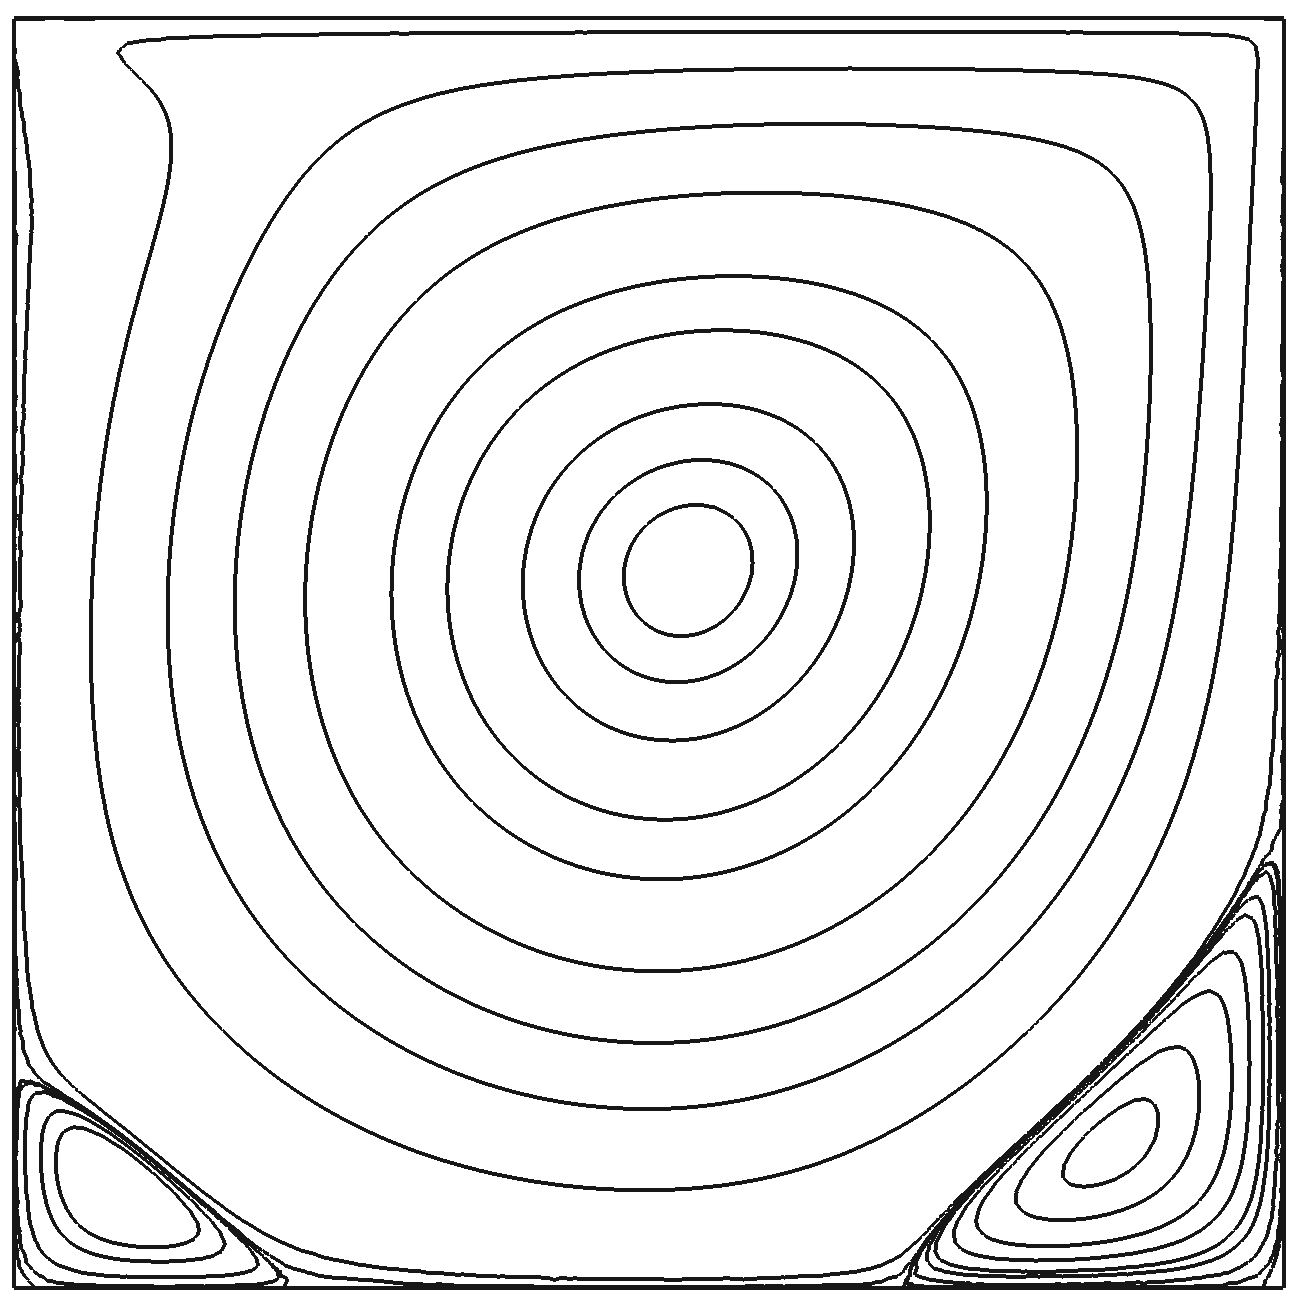
\includegraphics[width=0.4\textwidth]{./driven_cavity/driven_cavity_streamfunction.png}
\caption{Streamfunction contours in converged solution for $h=1/128$.}
\end{figure}
% end my slide
\end{frame}

\begin{frame}
    \frametitle{Lid--Driven Cavity}
\begin{figure}
\centering
\subfigure[vorticity contours in converged solution for \mbox{$h=1/128$}]{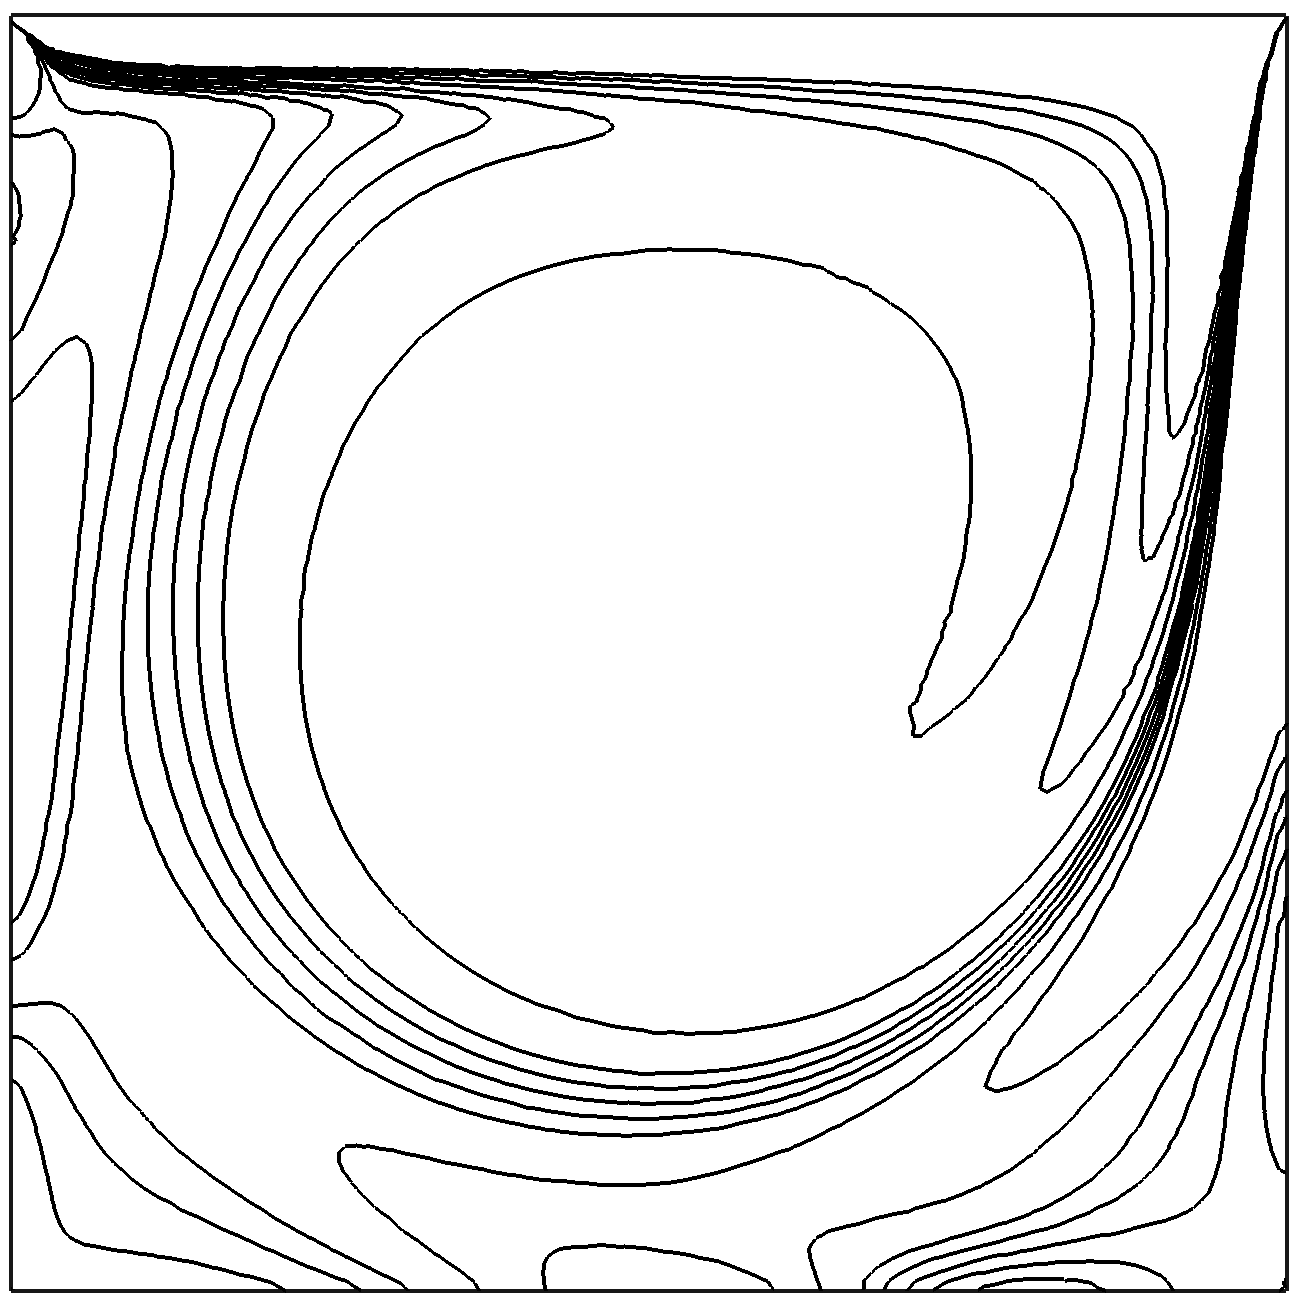
\includegraphics[width=0.35\textwidth]{./driven_cavity/driven_cavity_vorticity.png}}
\hspace{10mm}
\subfigure[error vs. experiment]{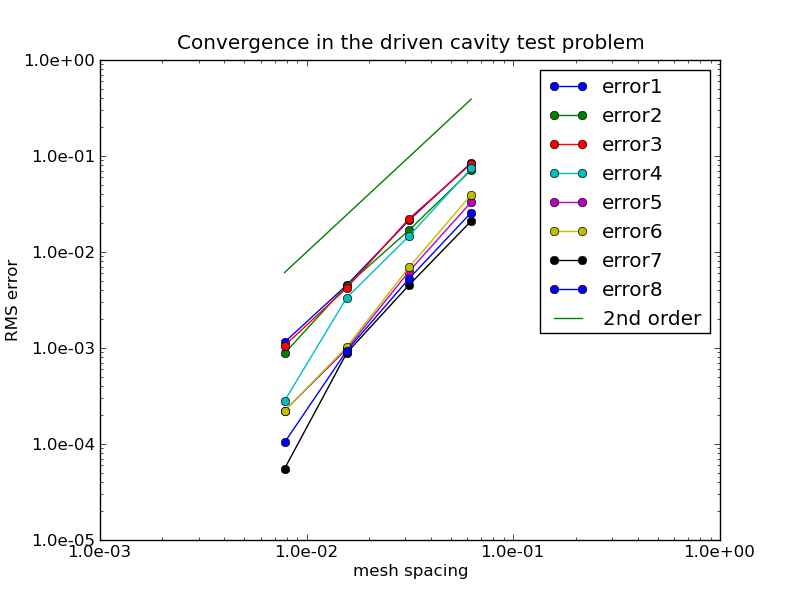
\includegraphics[width=0.45\textwidth]{./driven_cavity/driven_cavity_error_plot.png}}
\caption{The error metrics are listed in the manual.}
\end{figure}
\end{frame}





%-- Add sections and your outline will be created automatically --%
\subsection{Backward facing step}

\begin{frame}
    \frametitle{Backward facing step (2D and 3D)}
\begin{itemize}
\item Classic CFD test case
\item Experimental and numerical data available for comparison
\item Test of numerical methods or turbulence models
\end{itemize}
\begin{figure}
\centering
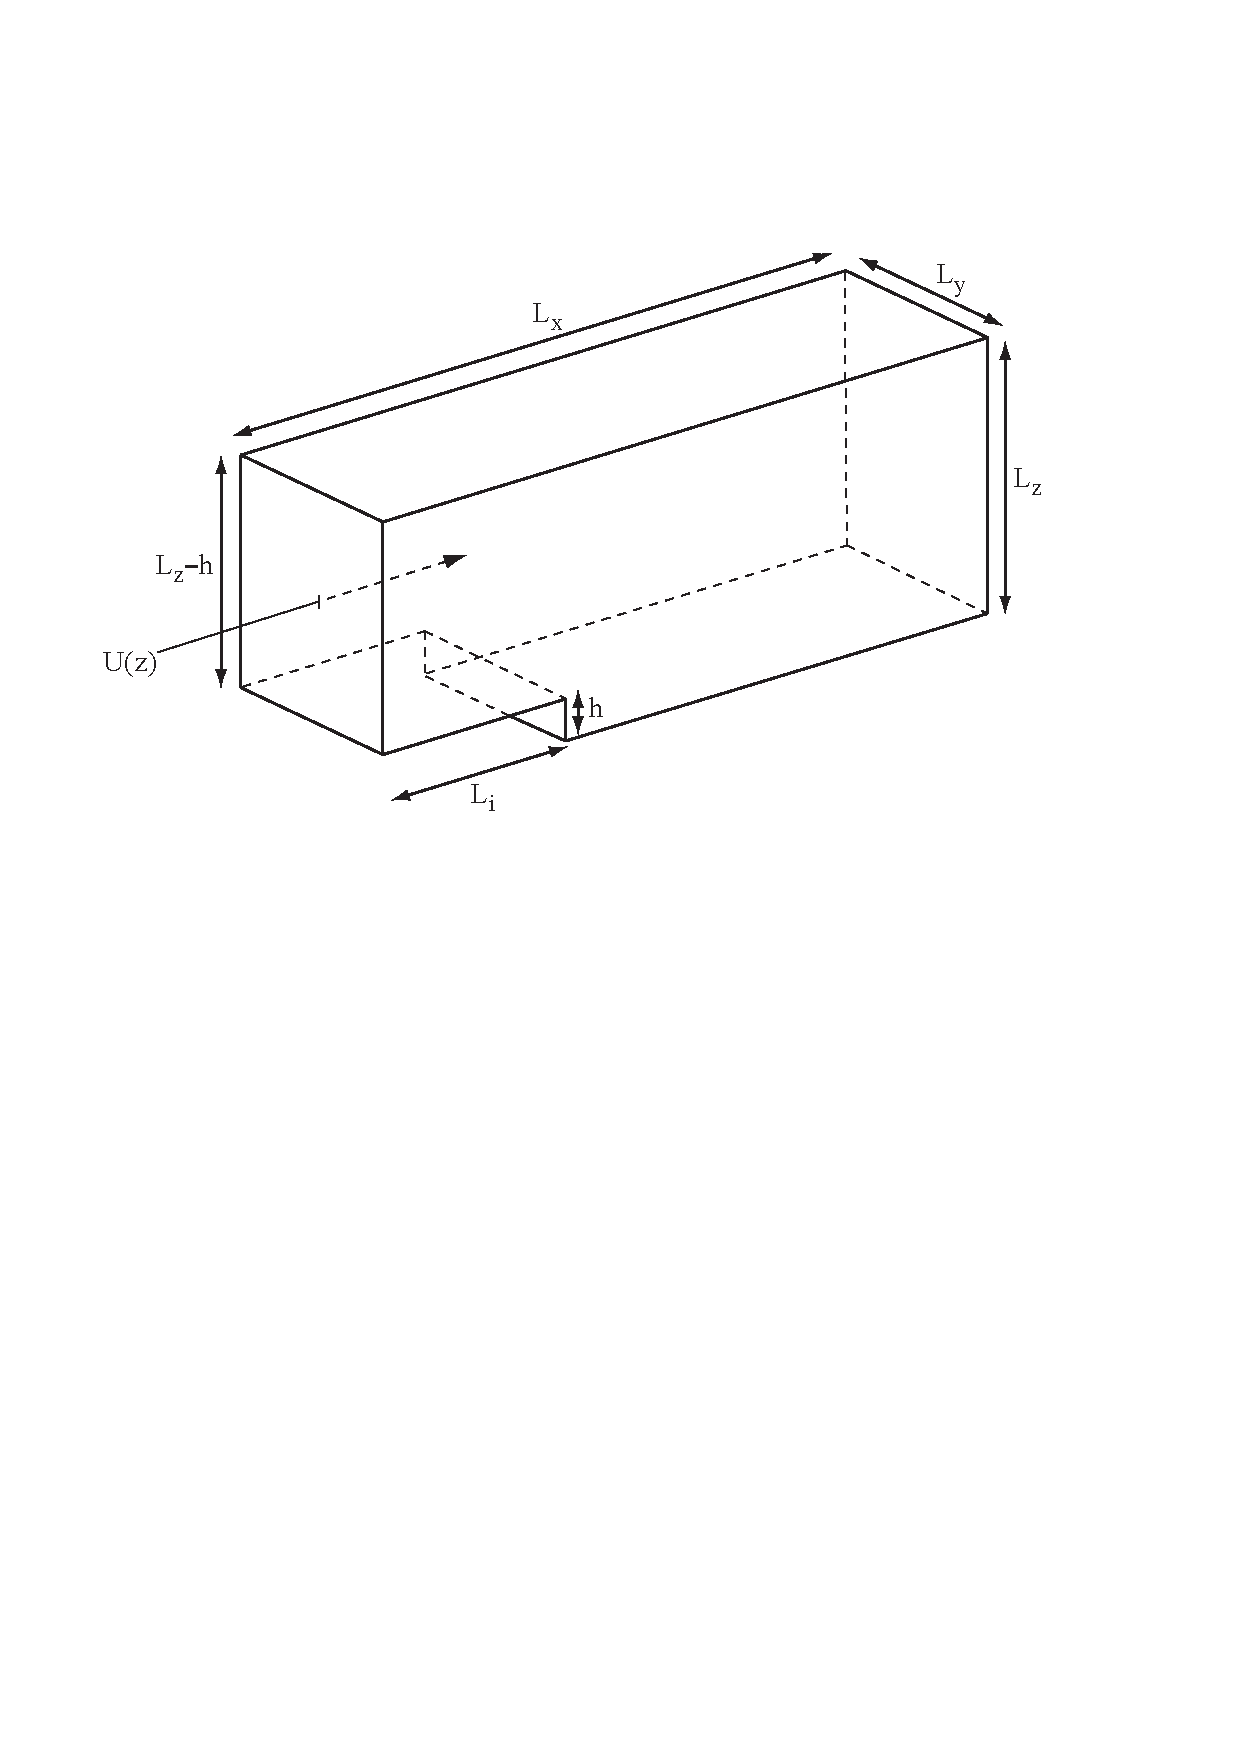
\includegraphics[width=0.5\textwidth]{./backward_facing_step/backward_facing_step_3d-schematic}
\caption{Geometry of 3D backward facing step}
\end{figure}
\end{frame}
%
\begin{frame}
    \frametitle{Backward facing step (2D and 3D)}
Run times: 
\begin{itemize}
\item 25 min. for 2D reference
\item 6 hr. for 2D with k-$\epsilon$
\item 5 hr. (8 cpu) for 3D
\end{itemize}
\begin{figure}
\centering
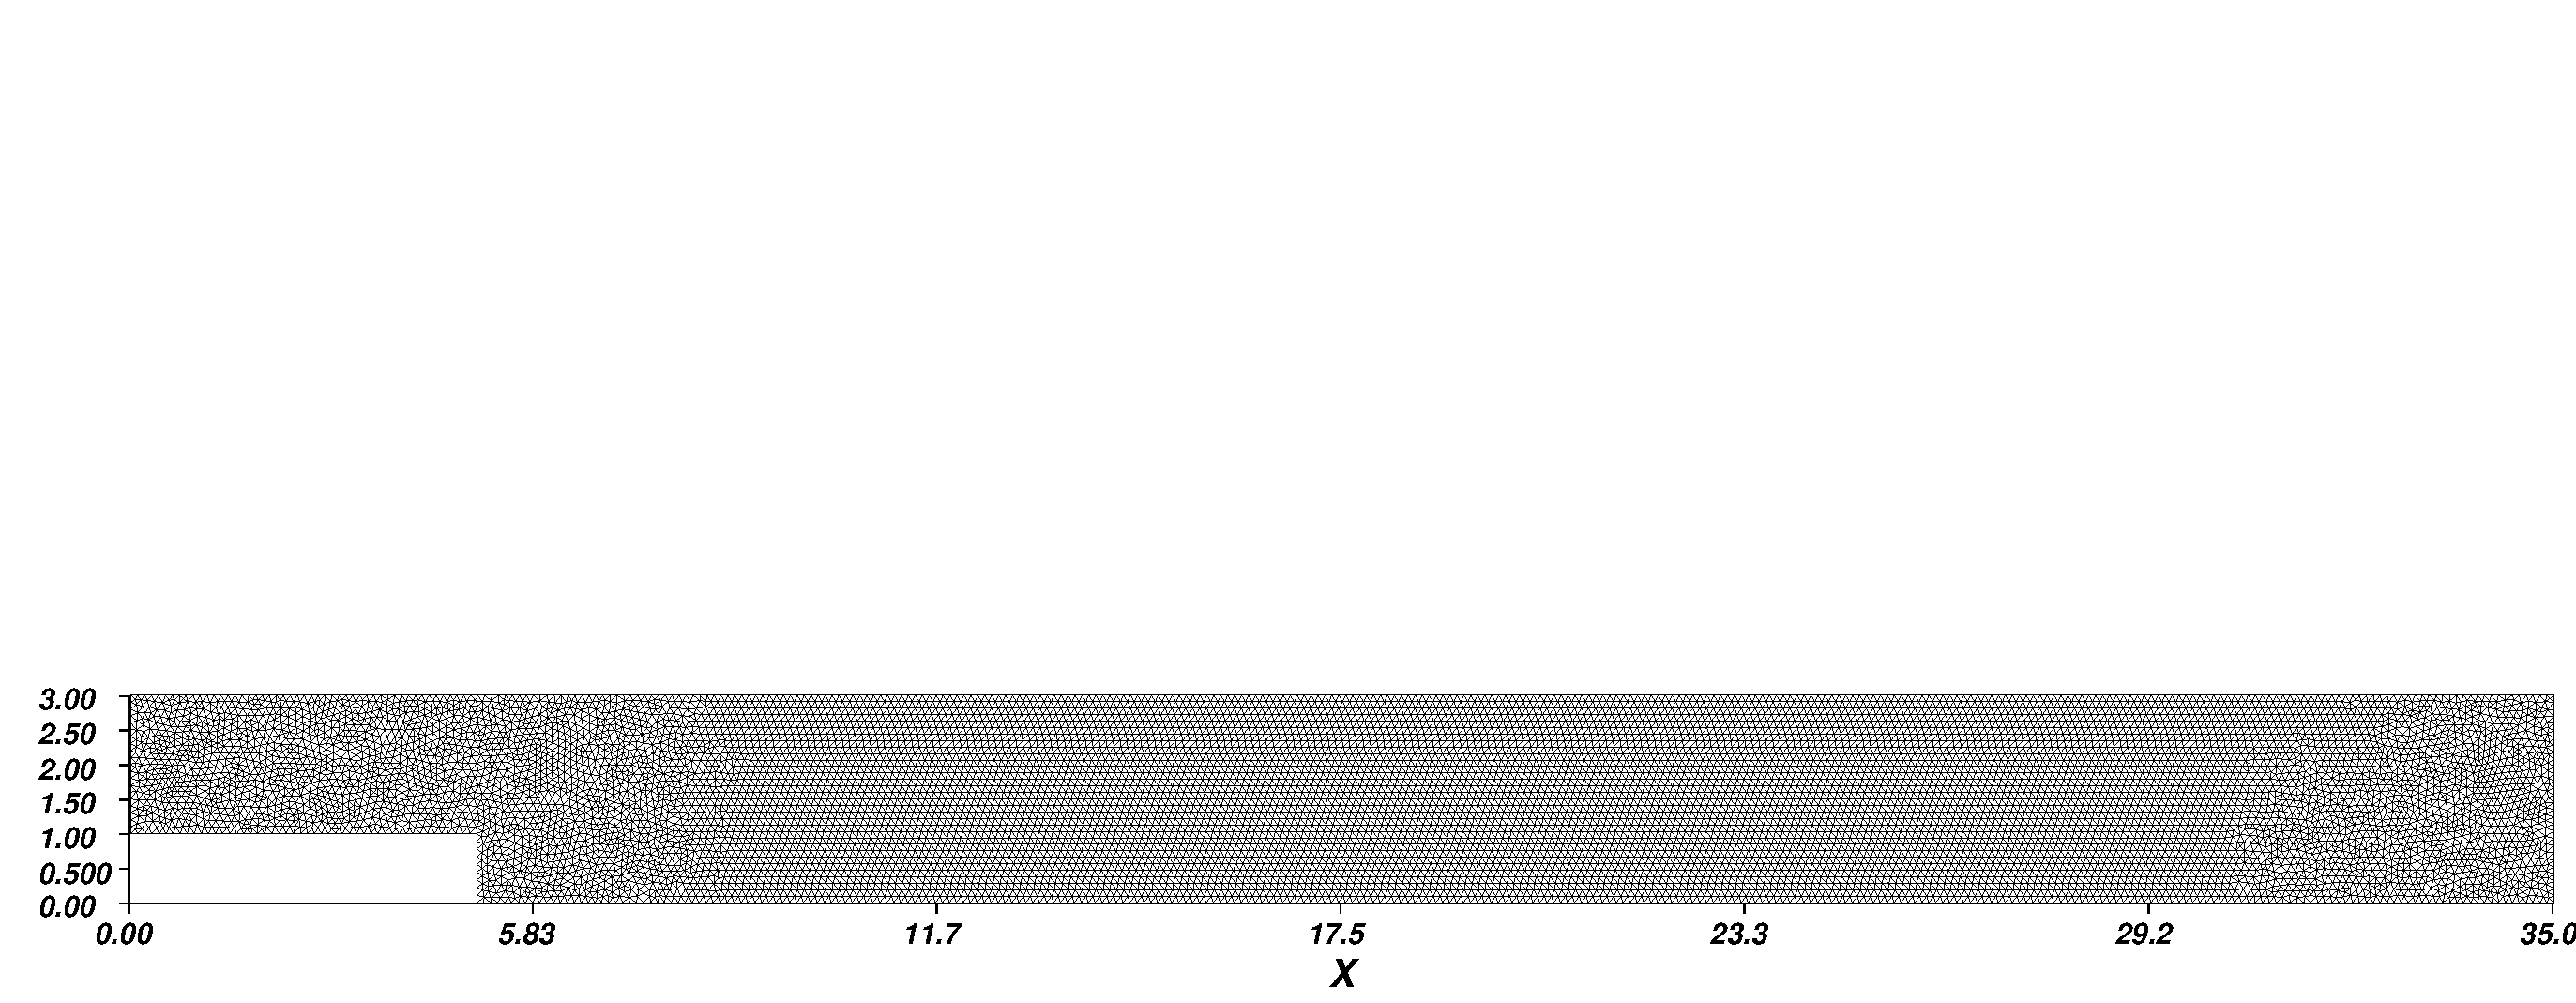
\includegraphics[width=1.0\textwidth]{./backward_facing_step/backward_facing_step_2d-mesh}
\caption{Geometry of 2D backward facing step showing the mesh.}
\end{figure}
\end{frame}
%
\begin{frame}
    \frametitle{Backward facing step, 2D results}
\begin{itemize}
\item Reattachment point estimation
\item Profile evolution in time/space
\end{itemize}
\begin{figure}
\centering
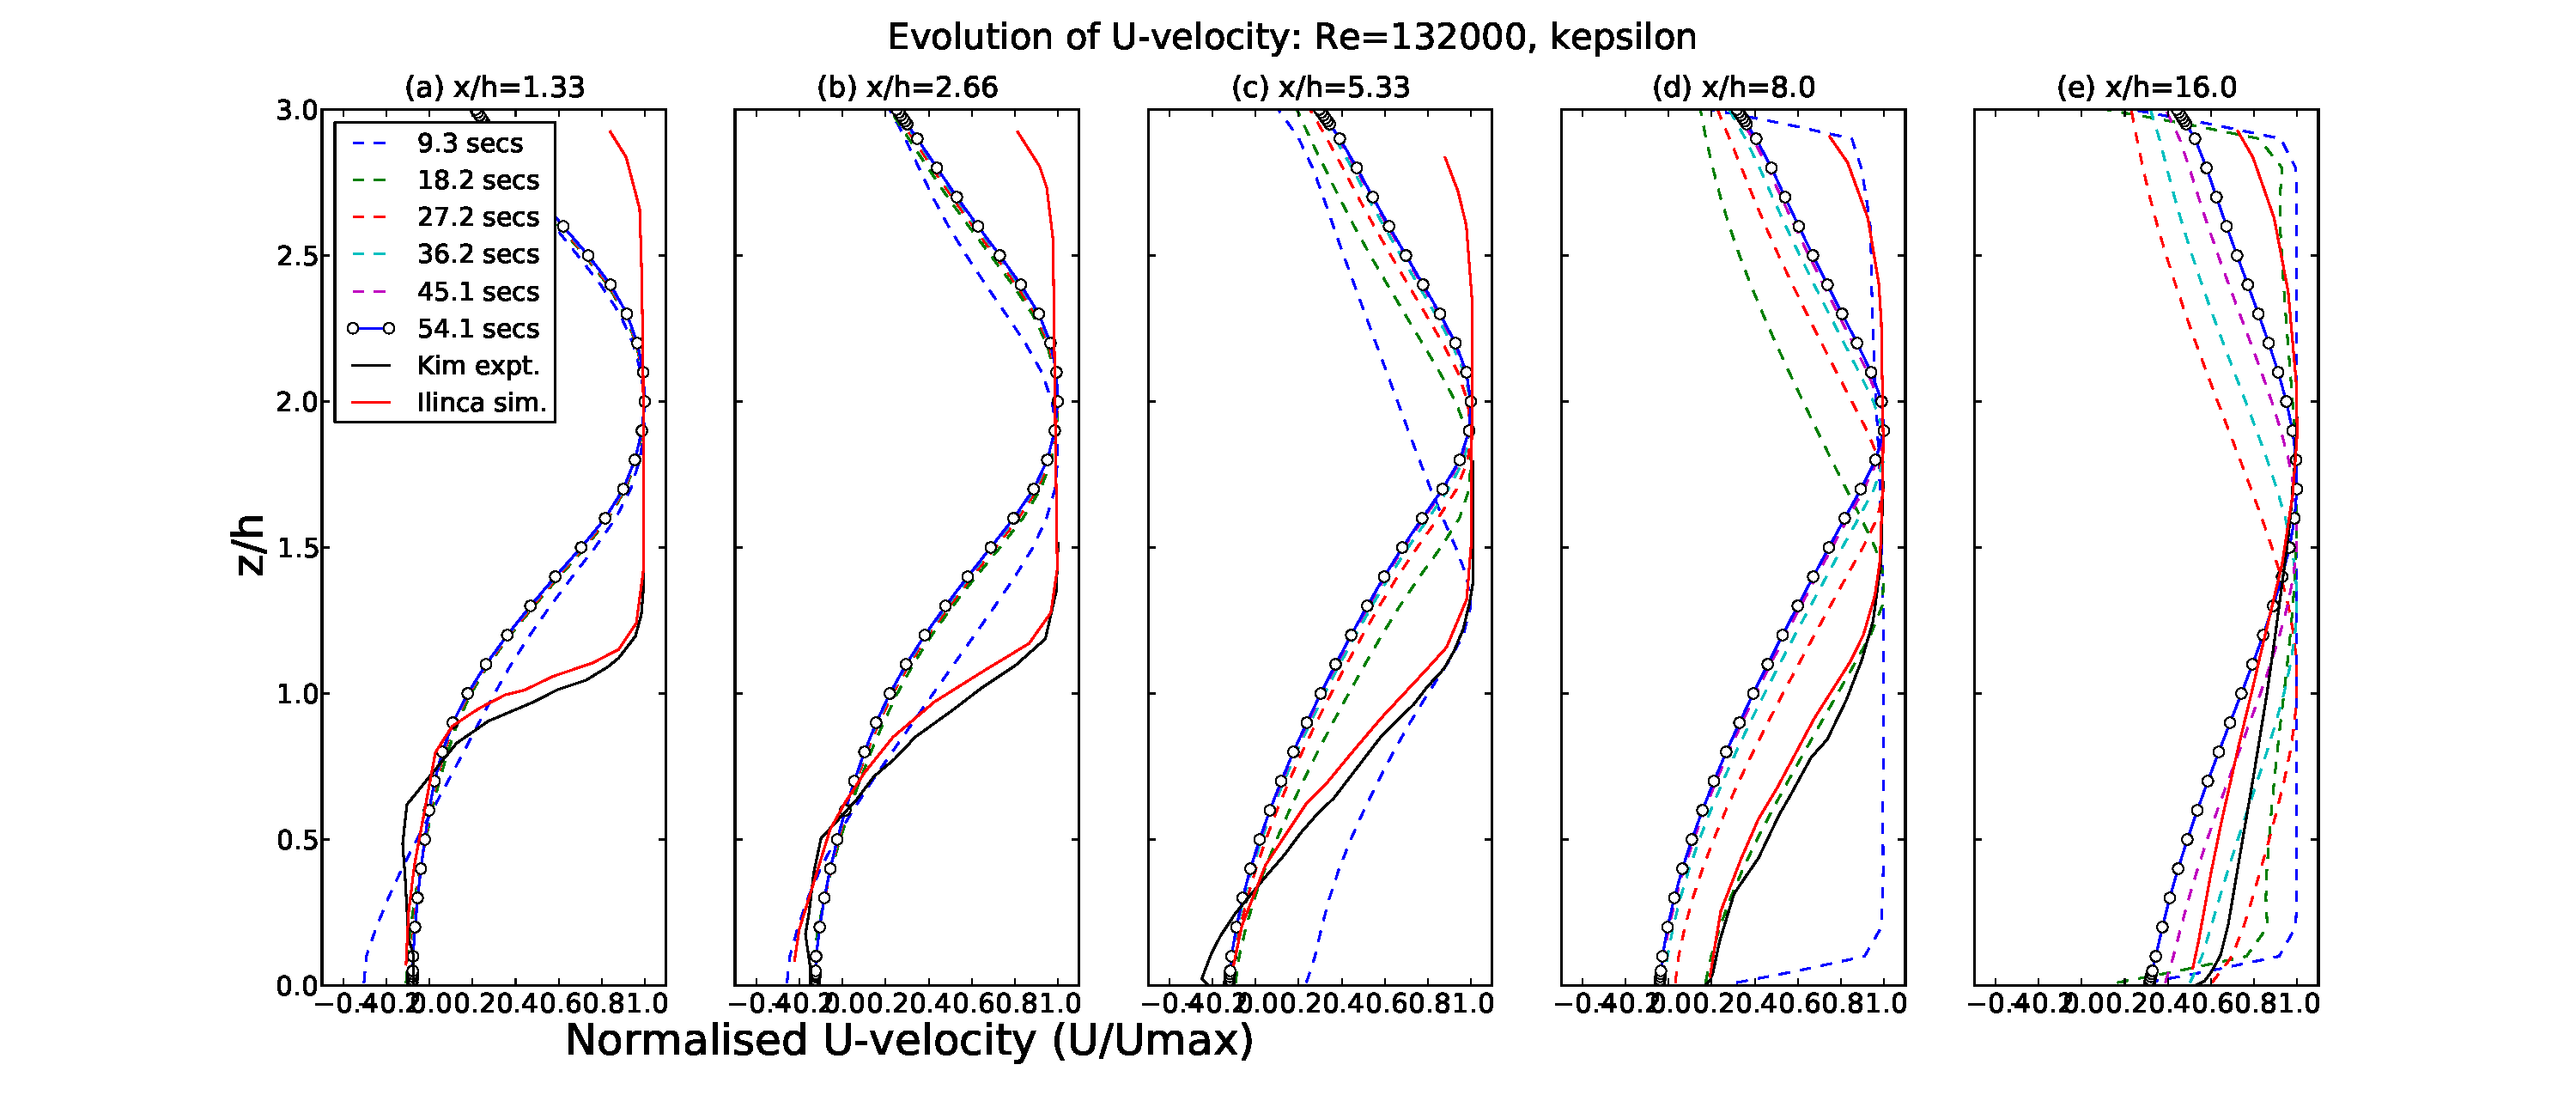
\includegraphics[width=0.7\textwidth]{./backward_facing_step/velocity_profiles_kim_kepsilon}
\caption{Streamwise velocity profiles at several points downstream of the step showing the converged solution and comparing to experimental and other numerical data.}
\end{figure}

\end{frame}
%
\begin{frame}
    \frametitle{Backward facing step, 3D results}
\begin{itemize}
\item Recirculation bubble and reattachment point
\end{itemize}

\begin{figure}
\centering
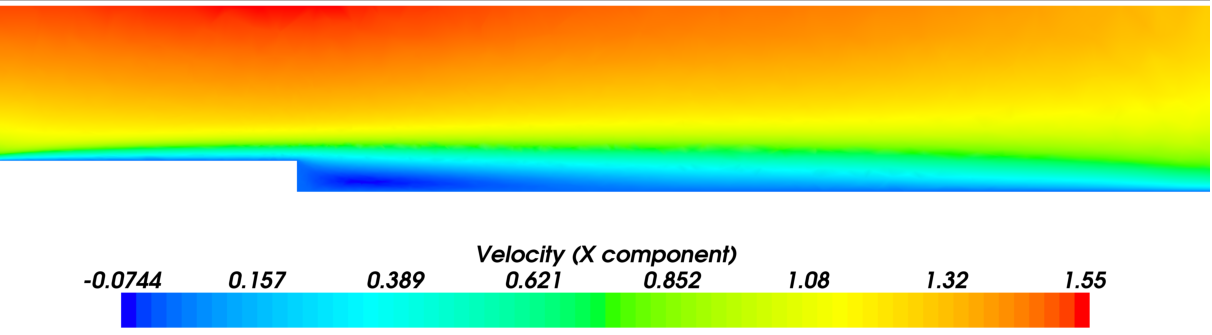
\includegraphics[width=0.8\textwidth]{./backward_facing_step/velo-magnitude-3d-50sec}
\caption{Velocity cut plane through centre of 3D geometry, time $=50\,$s.}
\end{figure}

\end{frame}
%
\begin{frame}
    \frametitle{Backward facing step, exercises}
\begin{itemize}
\item Increase the Reynolds number.
\item Add adaptivity options.
\end{itemize}

\end{frame}

%-- Add sections and your outline will be created automatically --%
\subsection{Flow past a sphere}

% Frame starts a new slide
\begin{frame}
    \frametitle{Flow past a sphere}
\begin{itemize}
\item Drag calculation at different Reynolds numbers
\item Adaptive mesh resolves dynamics near surface
%\item Option: \option{Velocity/stat/compute\_body\_forces\_on\_surfaces}
\end{itemize}
\begin{figure}
\centering
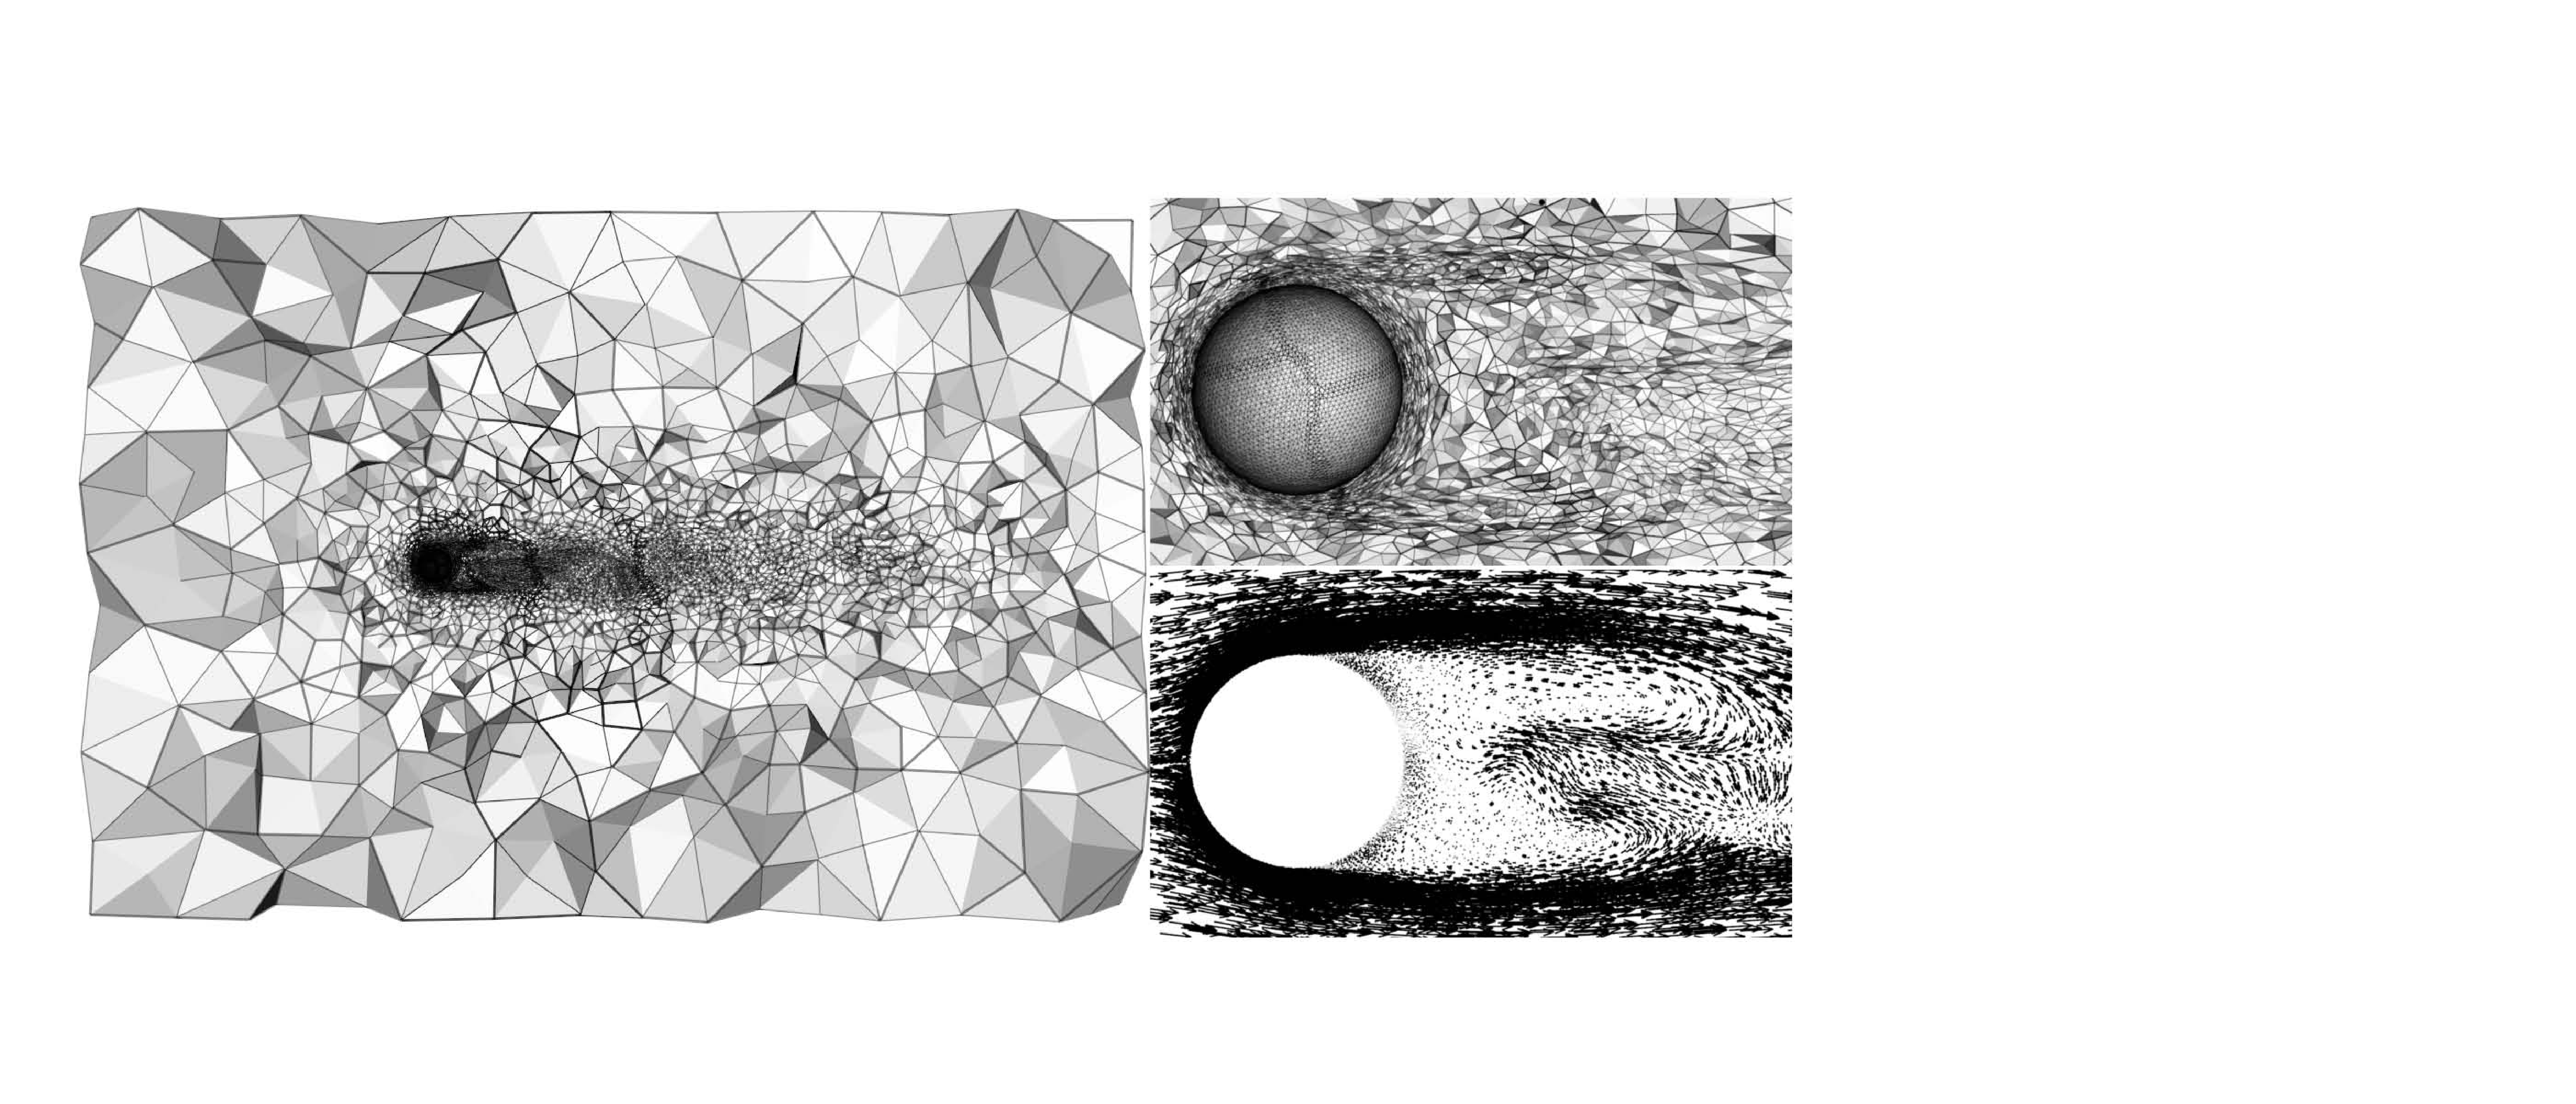
\includegraphics[width=0.8\textwidth]{./flow_past_sphere/sphere-Re1000-combined.pdf}
\caption{Sphere at $Re = 1000$. Clockwise from left: Cut plane showing anisotropic mesh, close up of sphere, velocity vectors.}
\end{figure}
\end{frame}

\begin{frame}
    \frametitle{Flow past a sphere}
\begin{itemize}
\item Plot streamlines by processing vtu files in Paraview
\item Time series of pressure and viscous drag force integrals available in stat file
%\item Option: \option{Velocity/stat/compute\_body\_forces\_on\_surfaces}
\end{itemize}
\begin{figure}
\centering
\subfigure[Re = 1]{
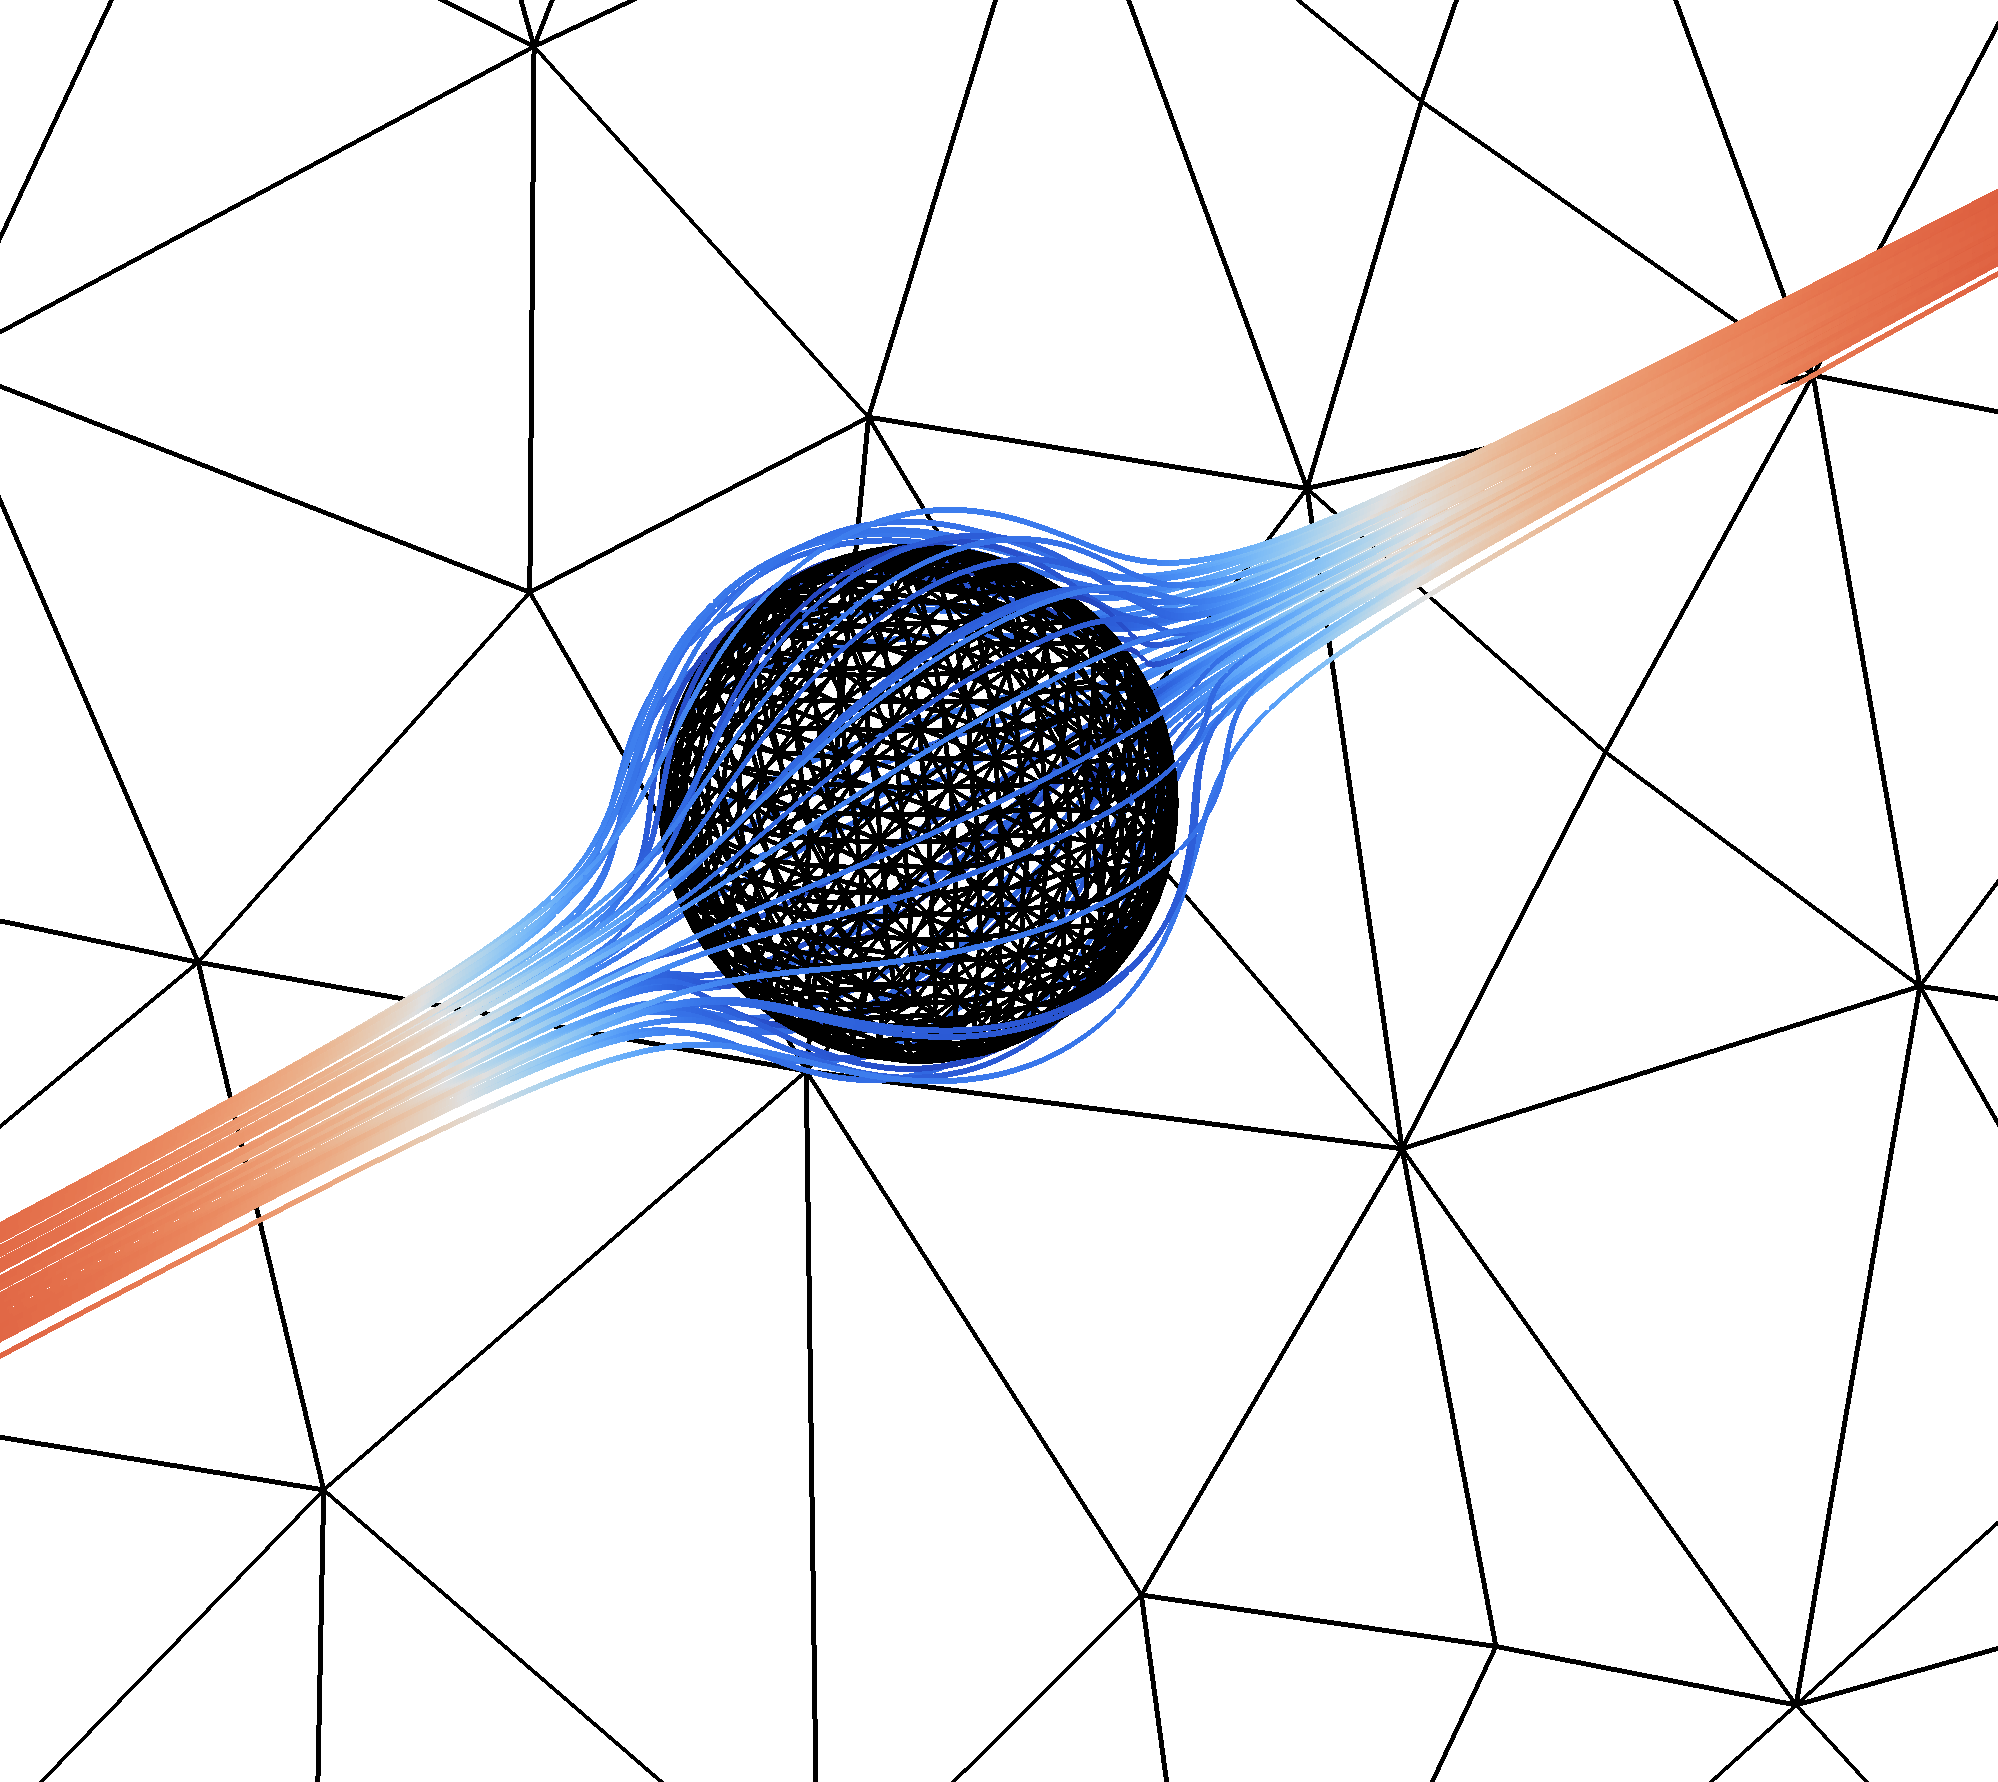
\includegraphics[width=0.225\textwidth]{./flow_past_sphere/sphere-Re1-streamlines.png}}
\subfigure[Re = 10]{
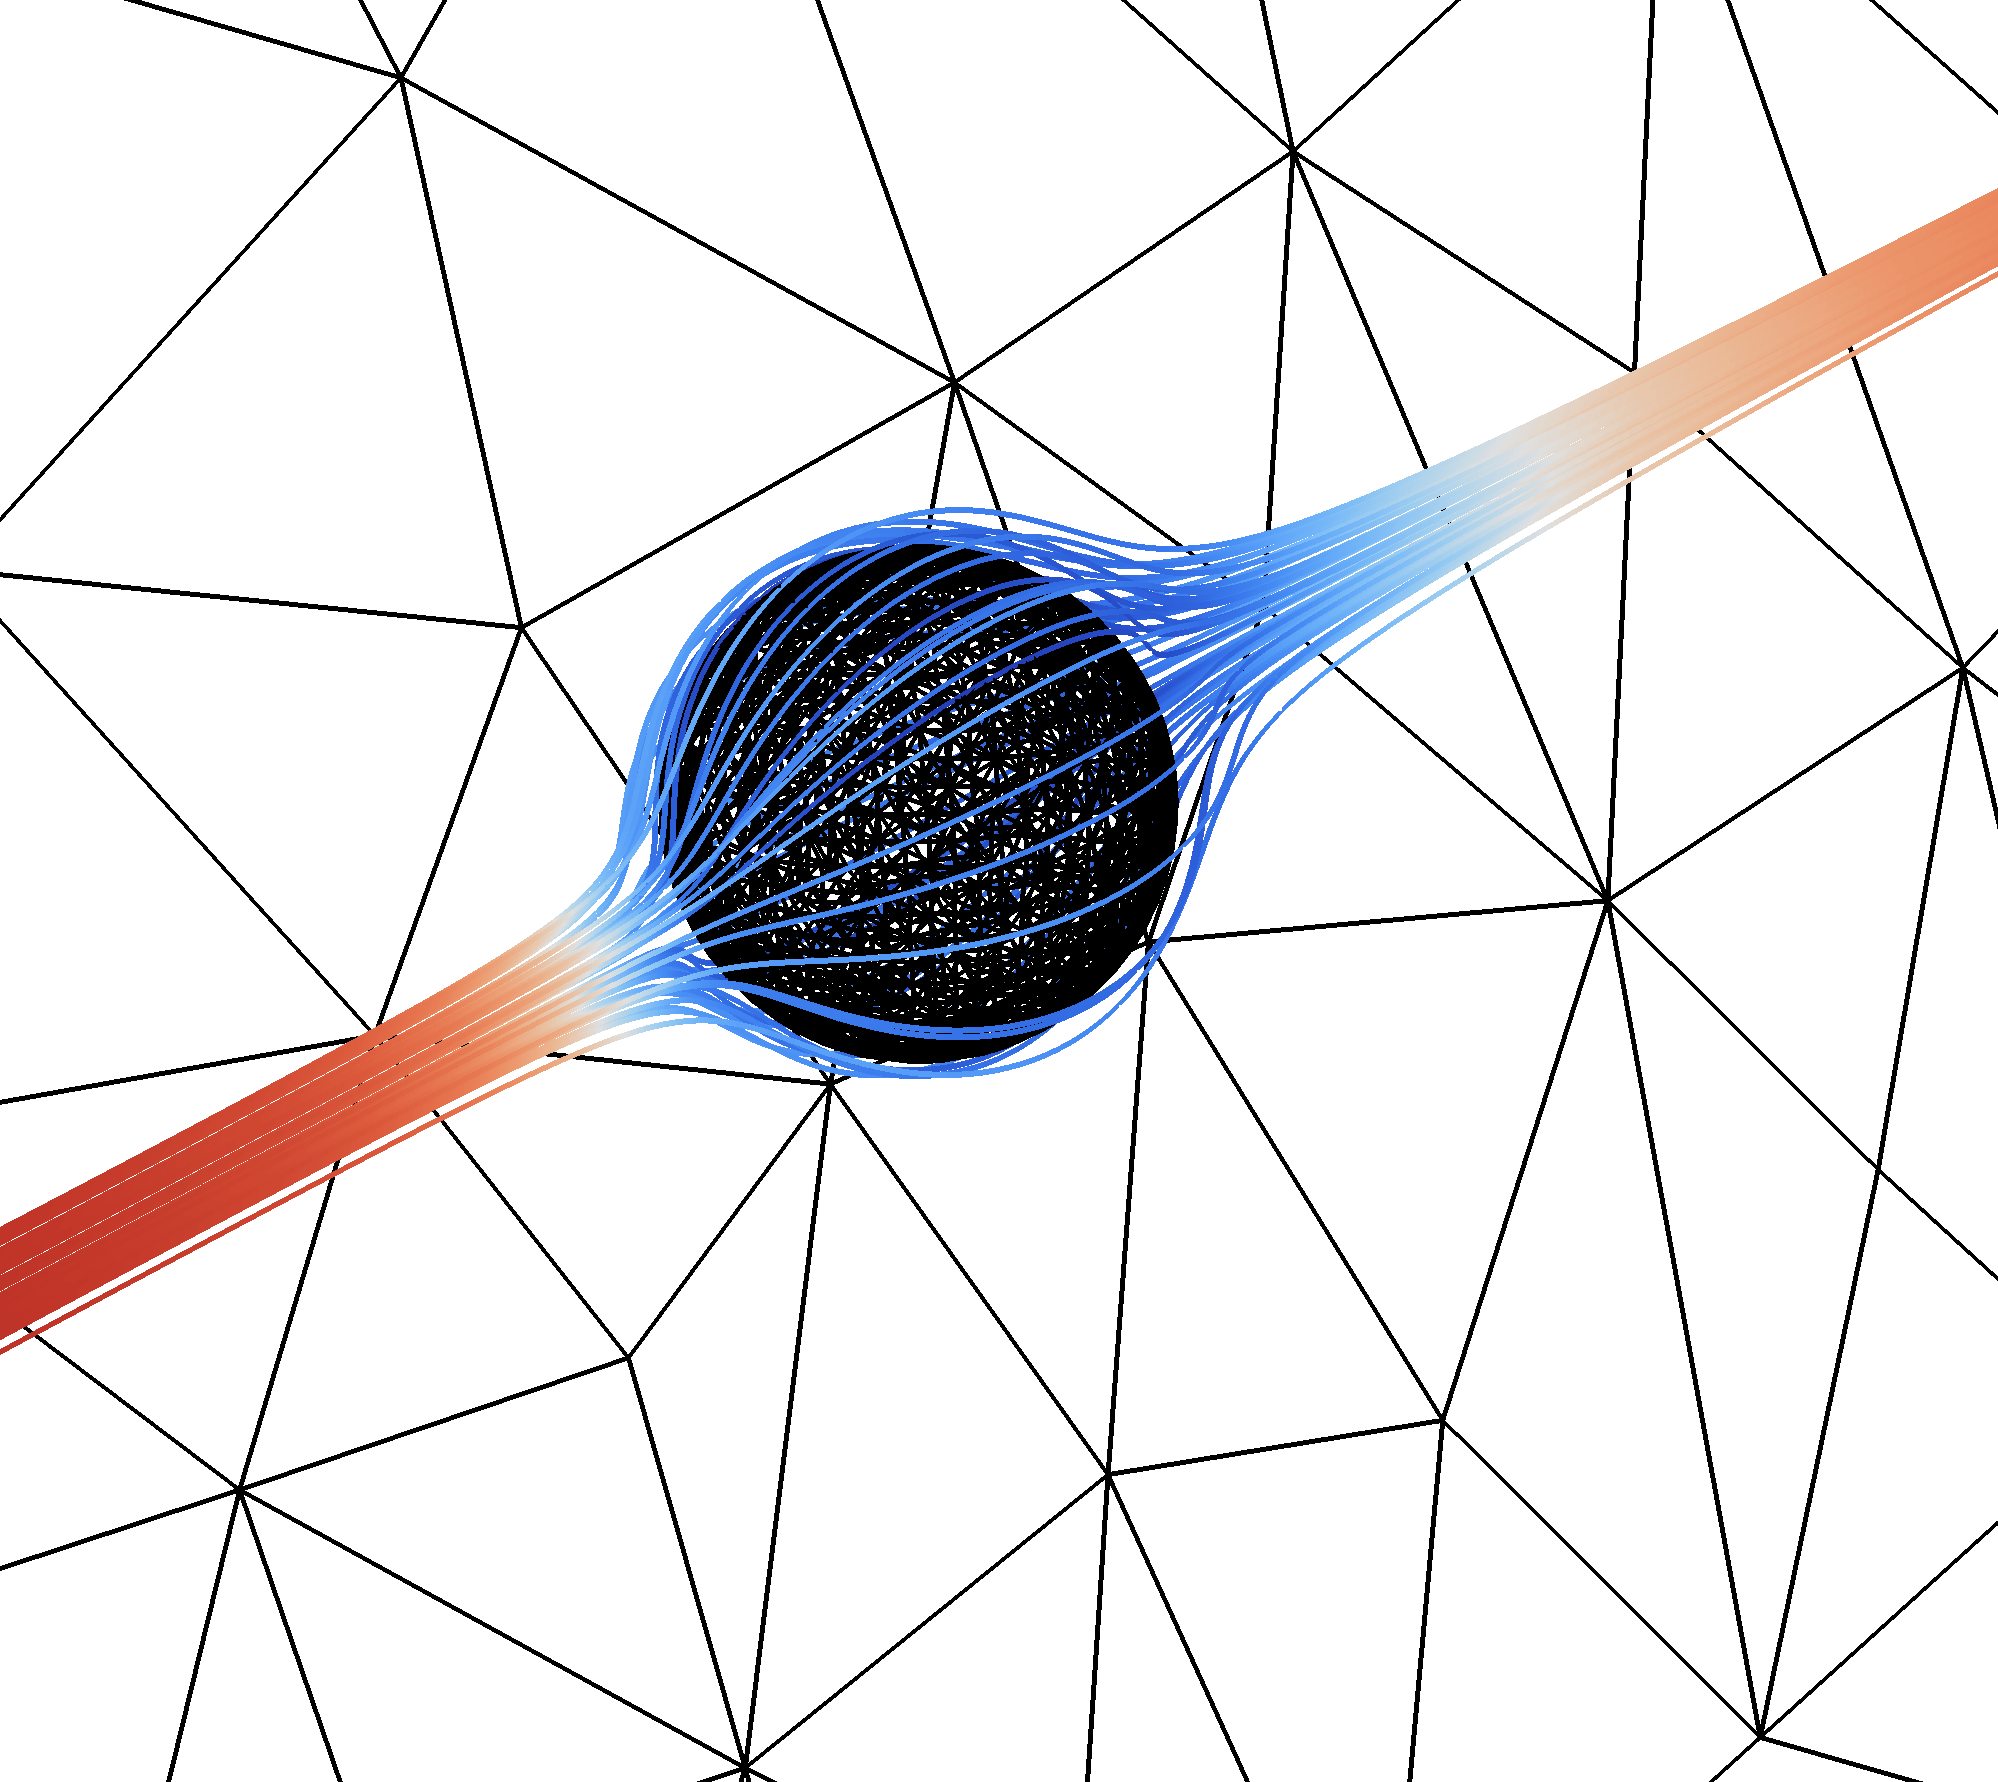
\includegraphics[width=0.225\textwidth]{./flow_past_sphere/sphere-Re10-streamlines.png}}
\subfigure[Re = 100]{
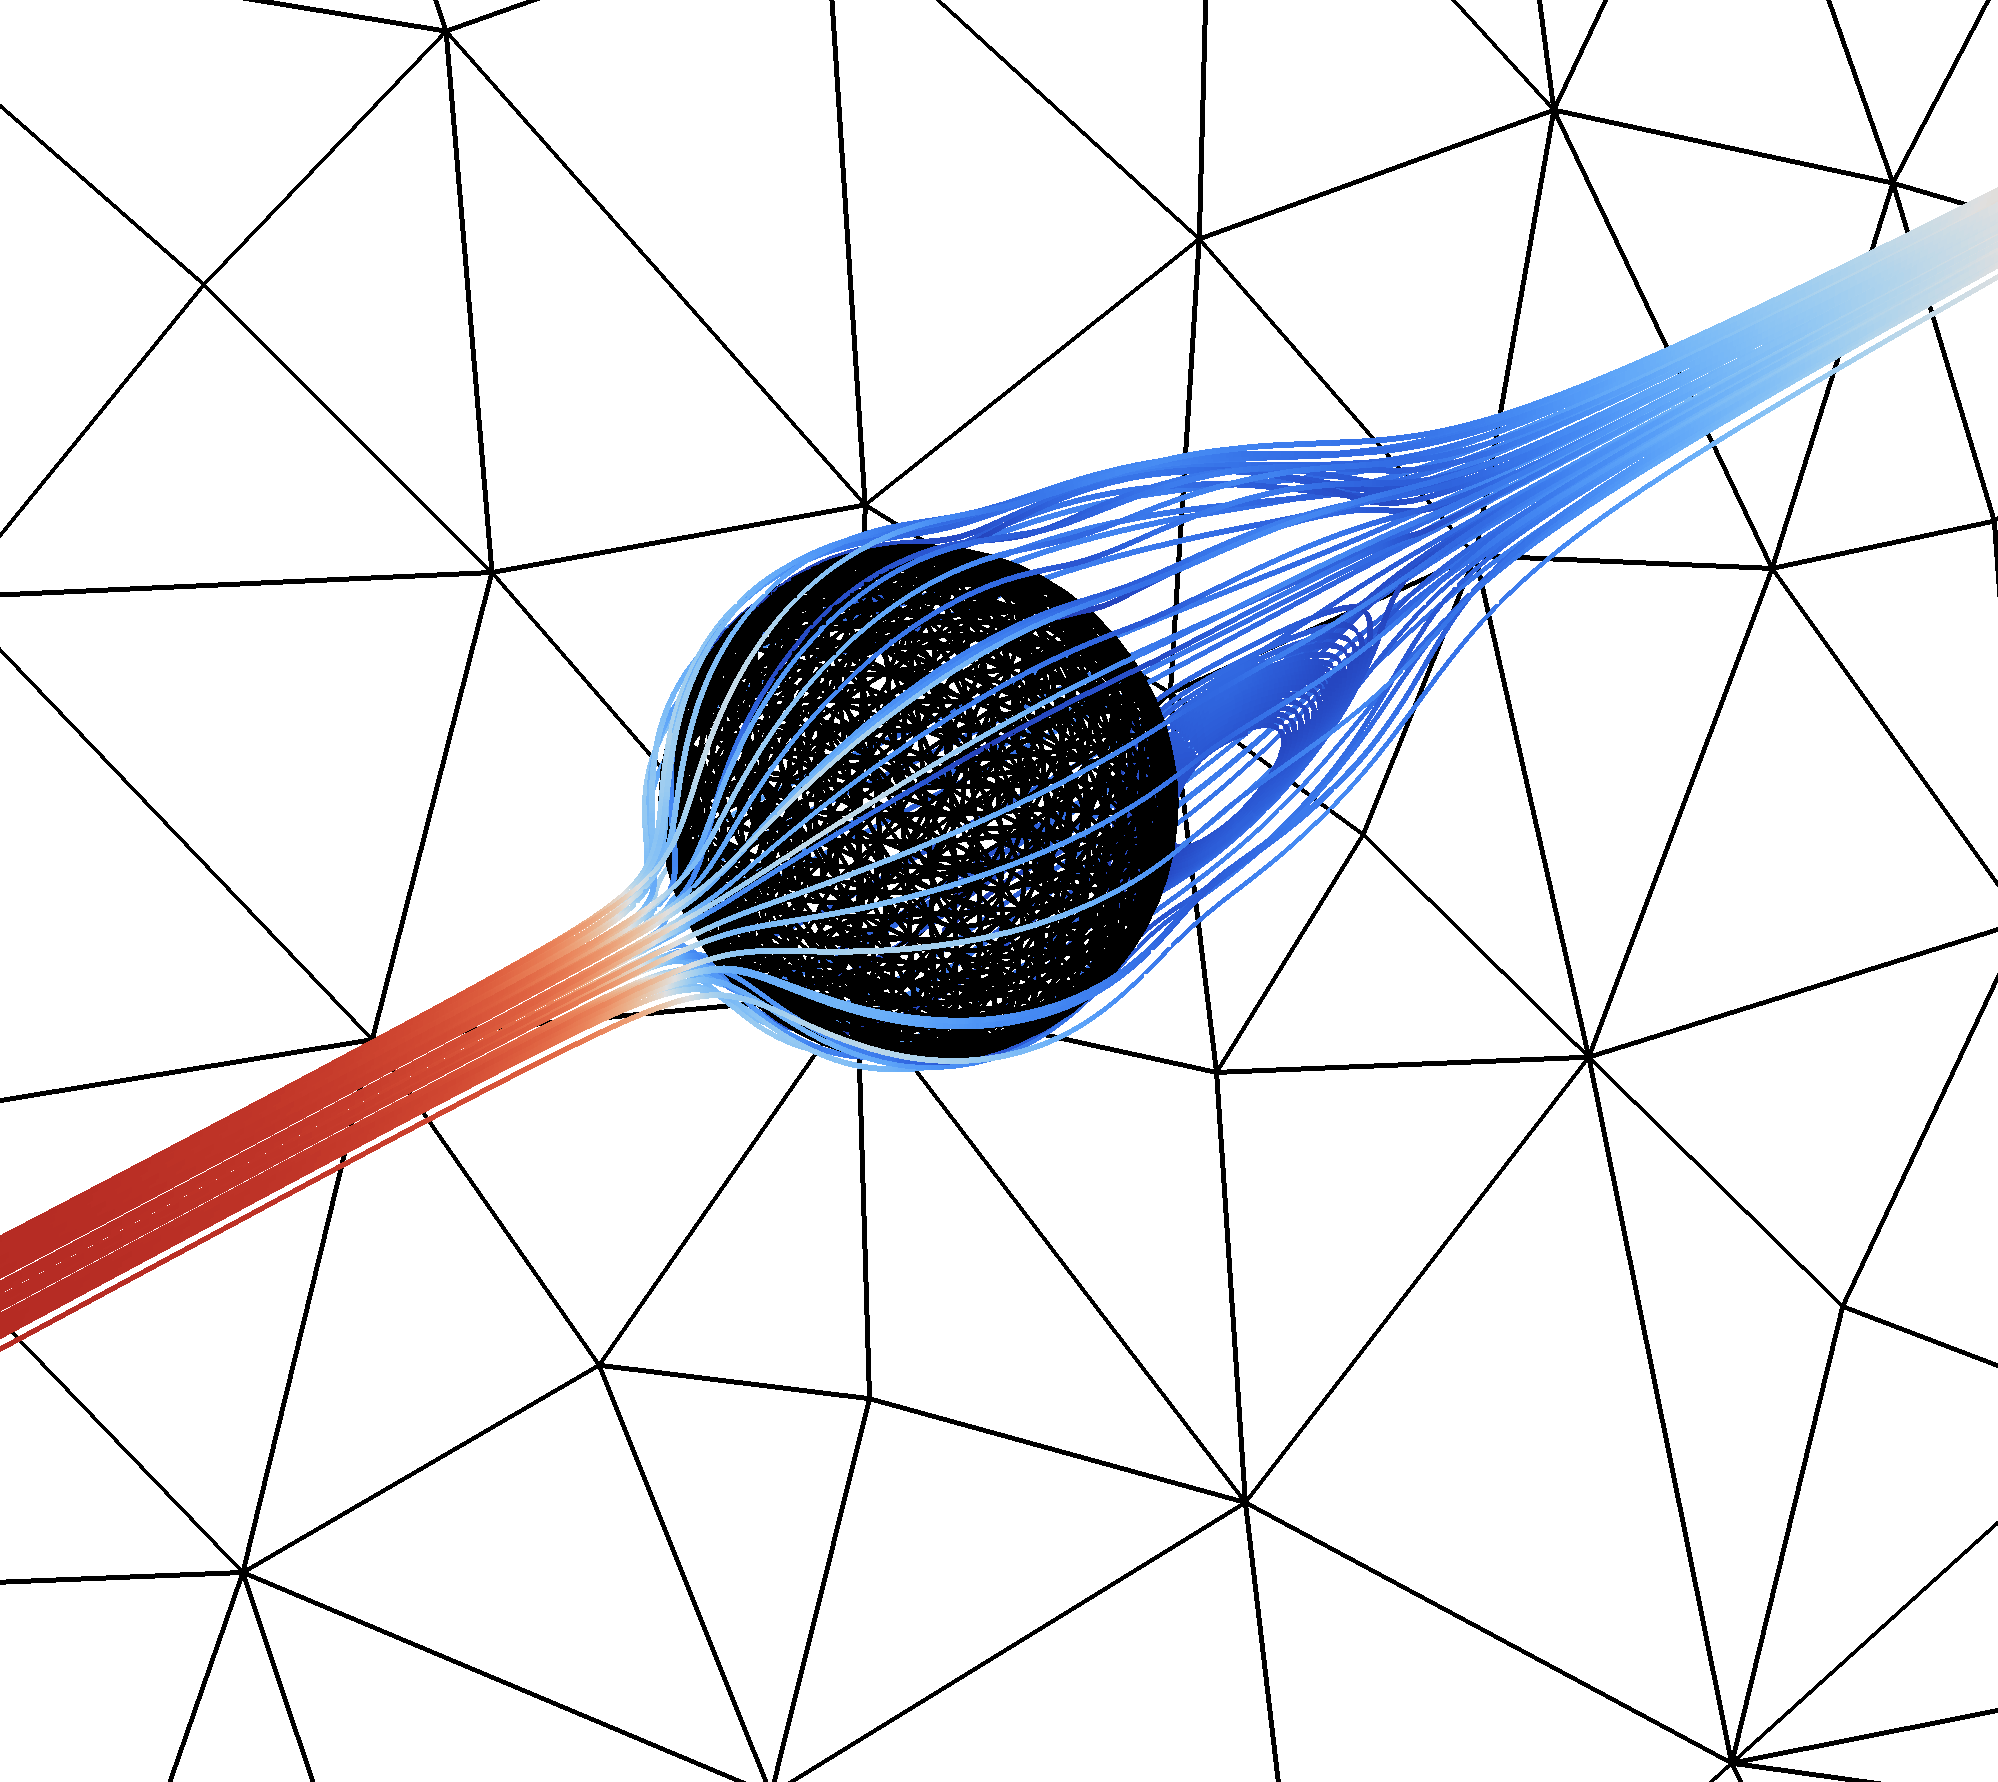
\includegraphics[width=0.225\textwidth]{./flow_past_sphere/sphere-Re100-streamlines.png}}
\subfigure[Re = 1000]{
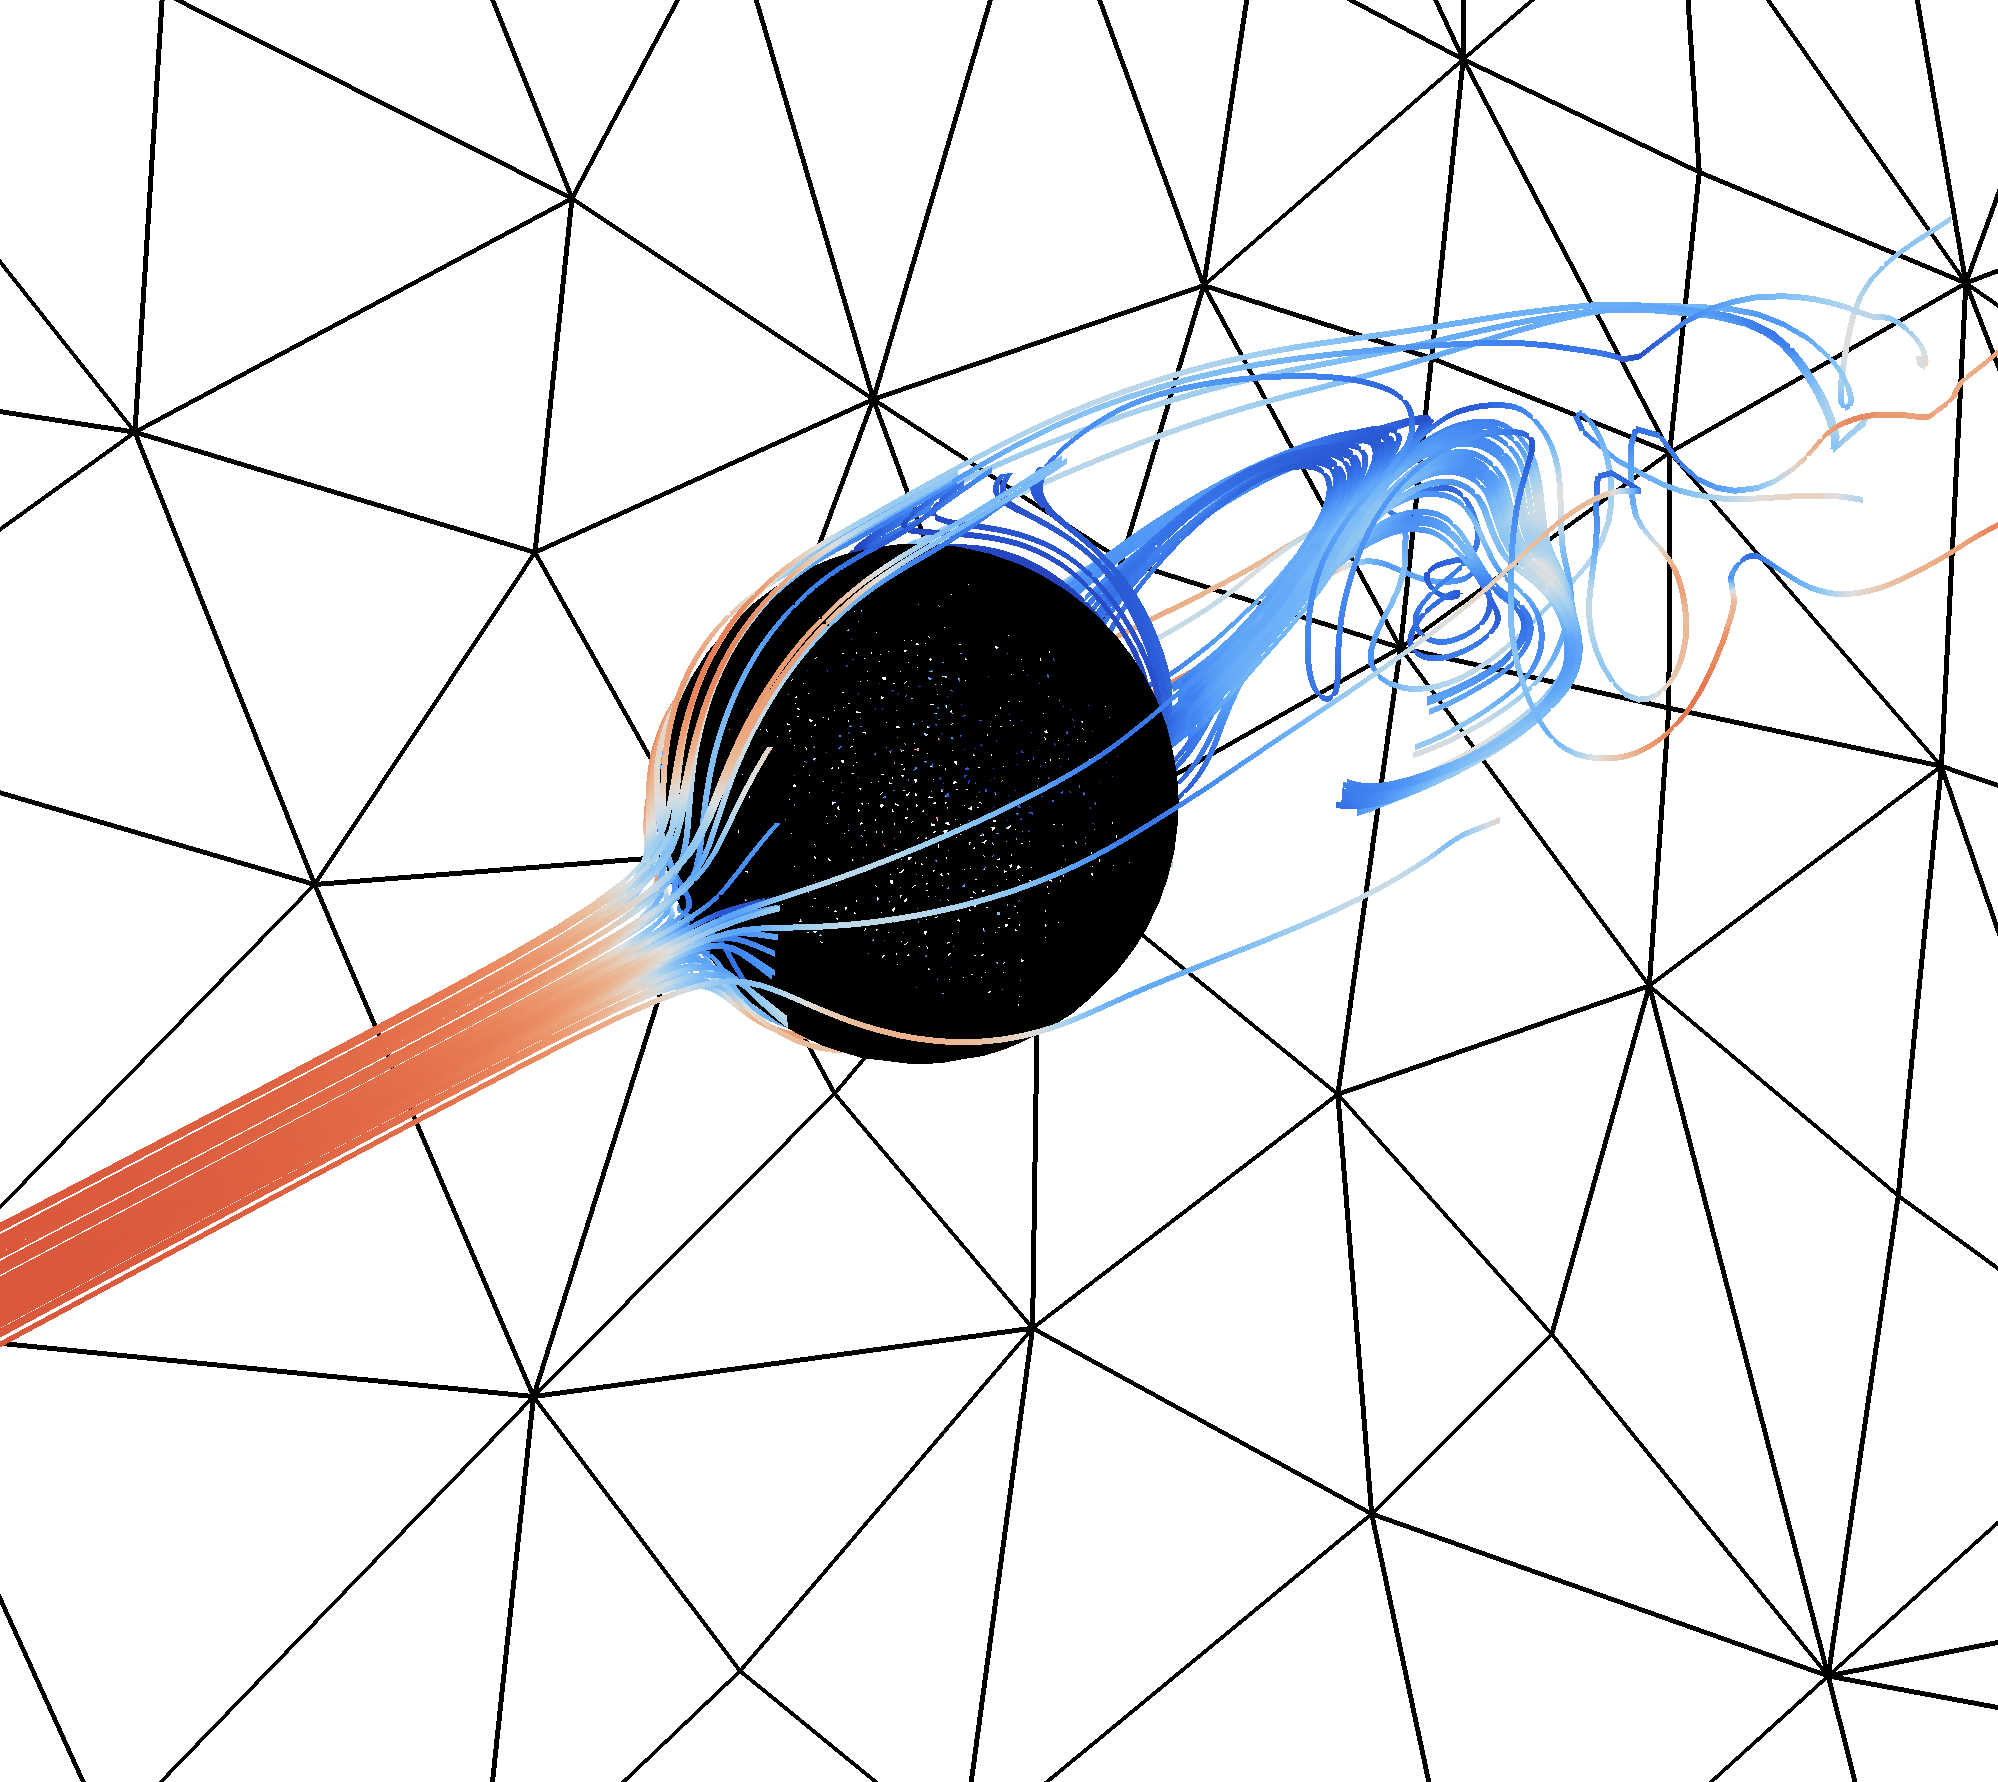
\includegraphics[width=0.225\textwidth]{./flow_past_sphere/sphere-Re1000-streamlines.png}}
\caption{Streamlines showing transition from laminar to turbulent wake with increasing Reynolds number.}
\end{figure}
\end{frame}

\begin{frame}
    \frametitle{Flow past a sphere}
\begin{figure}
\centering
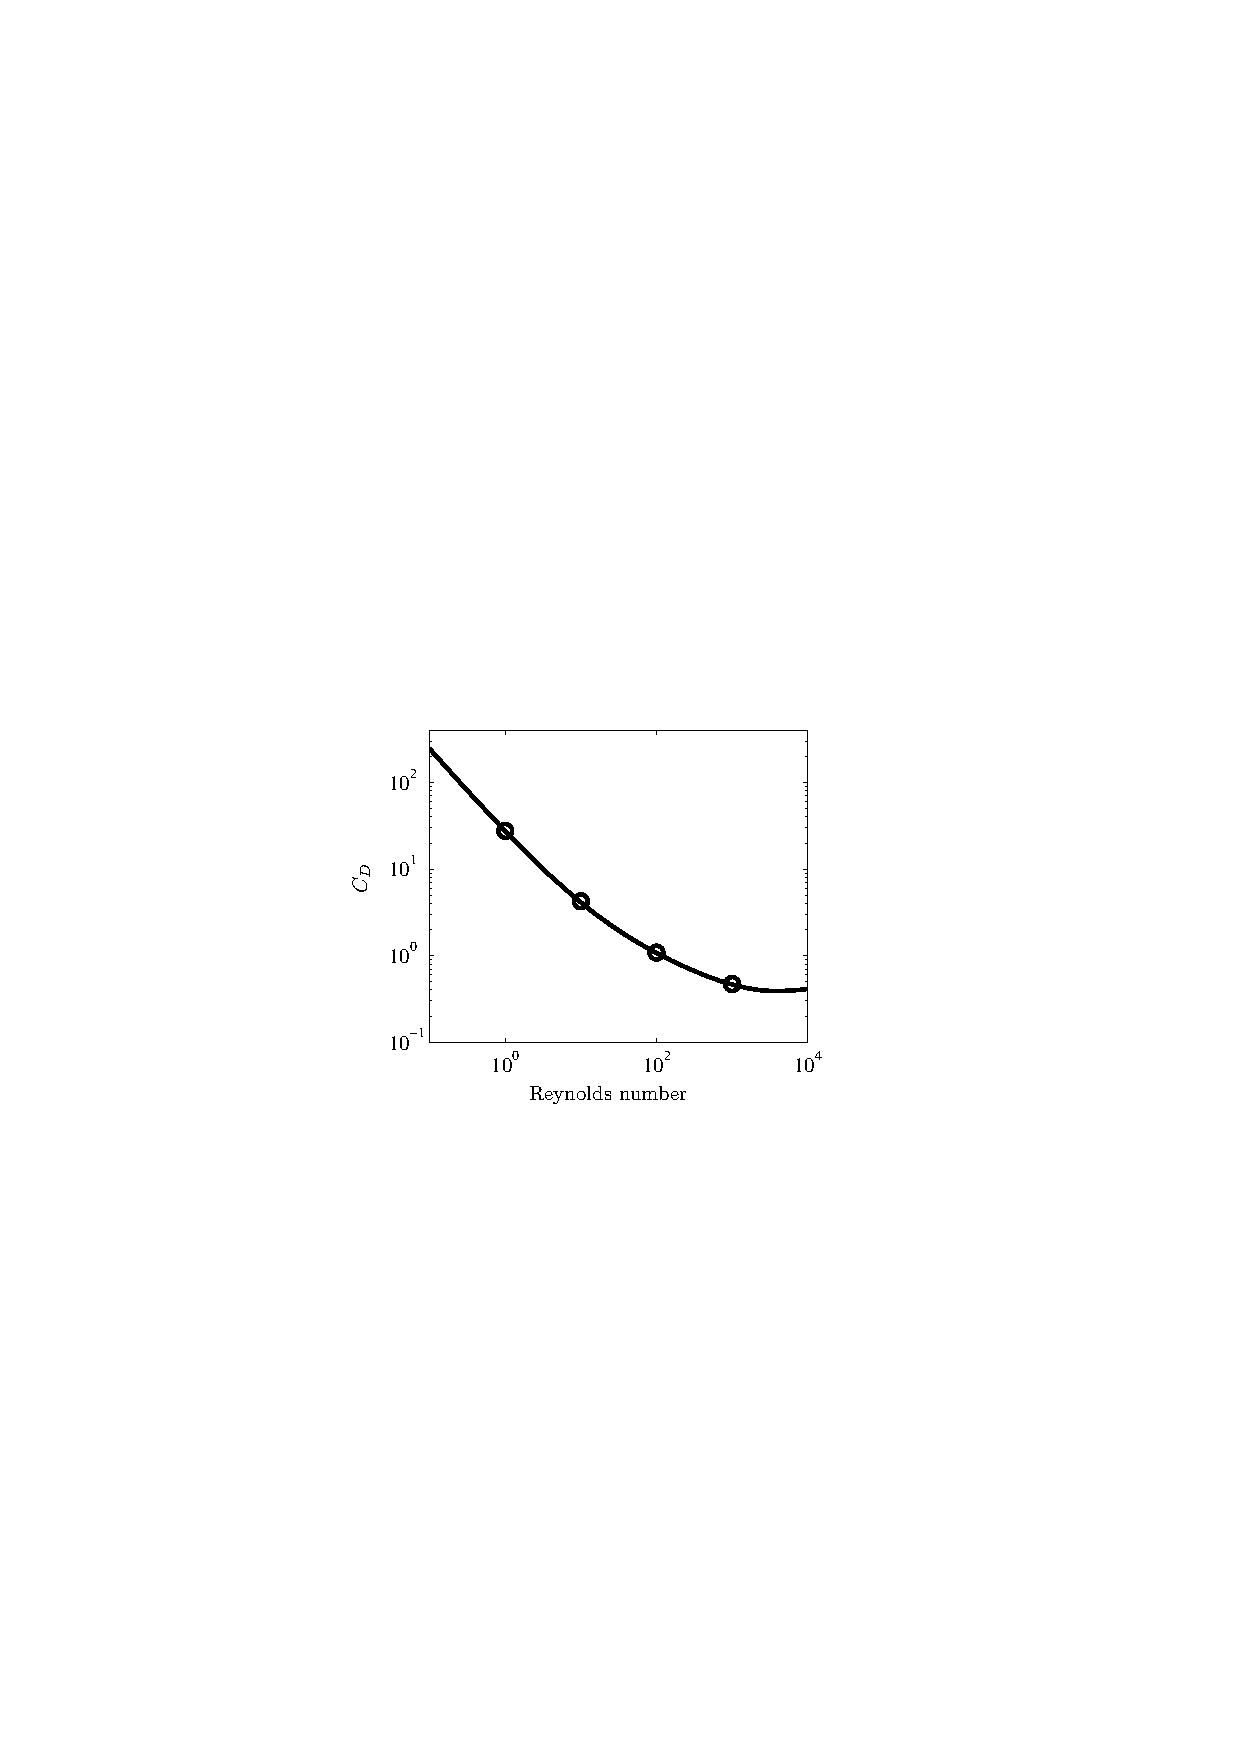
\includegraphics[width=0.5\textwidth]{./flow_past_sphere/Sphere_Drag.pdf}
\caption{Plot of drag coefficient vs. Reynolds number showing effect of turbulence. Circles: Fluidity data, line: correlation to experimental data from Brown and Lawler (2003), Journal of Environmental Engineering, 129(3).}
\end{figure}
\end{frame}

\begin{frame}
\frametitle{Flow past a sphere, exercises}
\begin{itemize}
\item Write an offline python diagnostic to calculate the drag.
\item Investigate impact different discretisations and adaptivity parameters on the drag.
\item Investigate different shaped objects.
\end{itemize}
\end{frame}

%-- Add sections and your outline will be created automatically --%
\subsection{Water collapse}

% Frame starts a new slide
\begin{frame}
    \frametitle{Water collapse}
\begin{itemize}
\item Multi--material problem: air, water
\item Compared to benchmark lab data
\item Barrier removed instantaneously at t = 0; flow driven by gravity
\end{itemize}

\begin{figure}
\centering
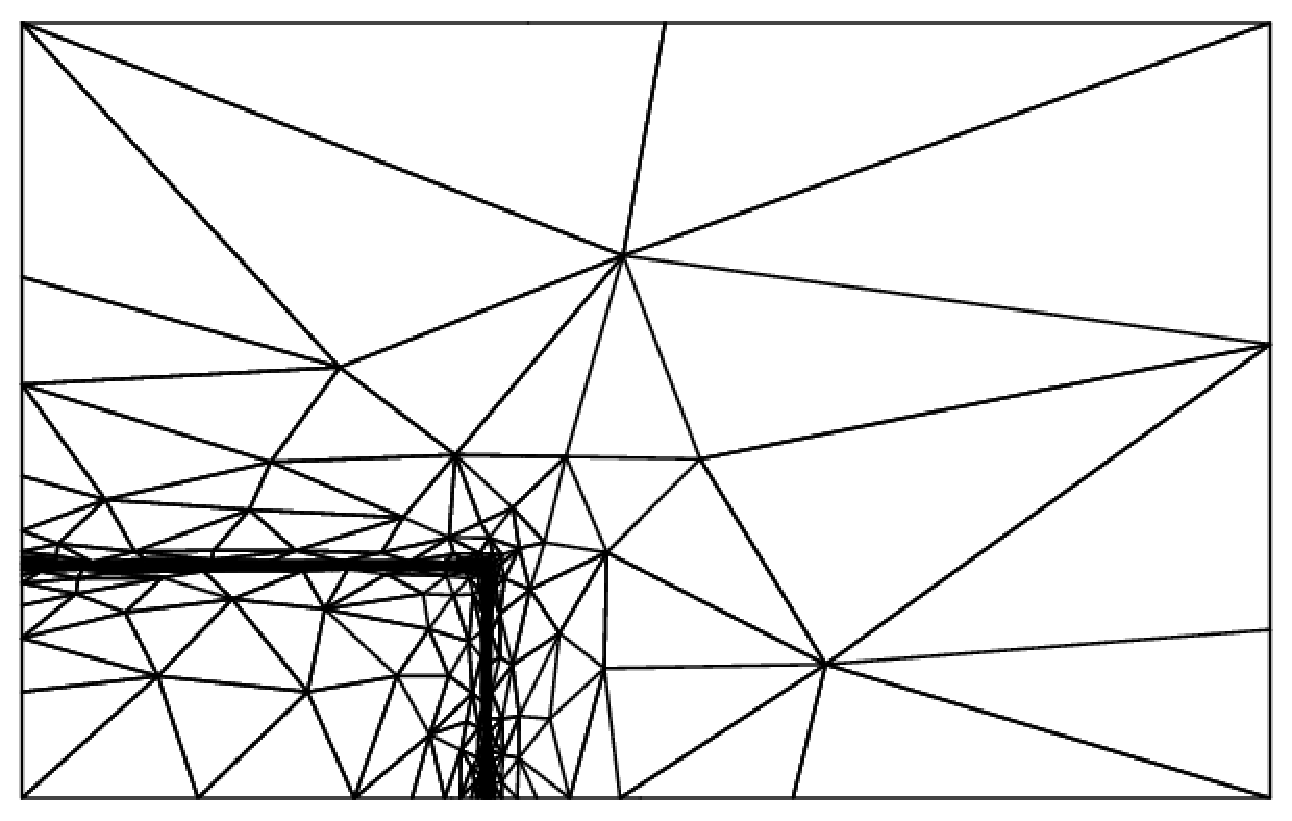
\includegraphics[width=0.6\textwidth, clip=true]{./water_collapse/water_collapse_0_mesh.pdf}
\caption{Initial unstructured adapted mesh for water collapse problem.}
\end{figure}

\end{frame}
%
\begin{frame}
    \frametitle{Water collapse}

\begin{figure}
\centering
\subfigure[$t=0.5$]{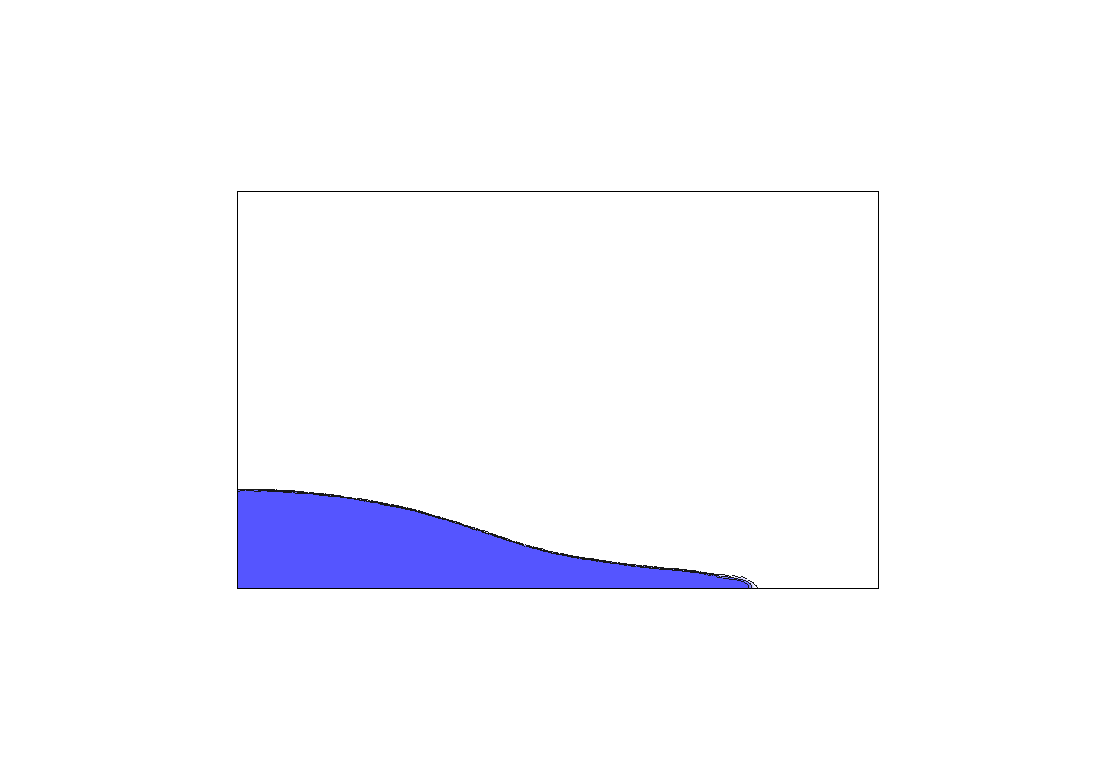
\includegraphics[width=0.275\textwidth, trim=7.5cm 6.5cm 7.5cm 6.5cm, clip=true]{./water_collapse/water_collapse_100.png}}
\subfigure[$t=1.0$]{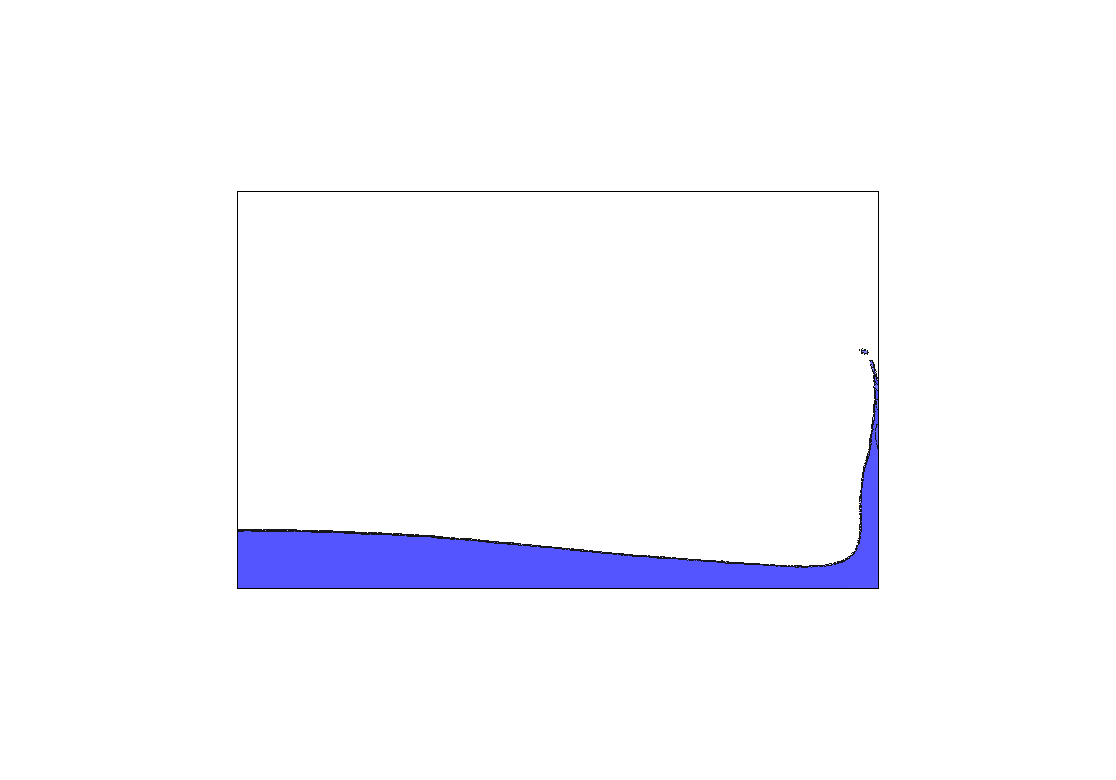
\includegraphics[width=0.275\textwidth, trim=7.5cm 6.5cm 7.5cm 6.5cm, clip=true]{./water_collapse/water_collapse_200.png}}
\subfigure[$t=1.5$]{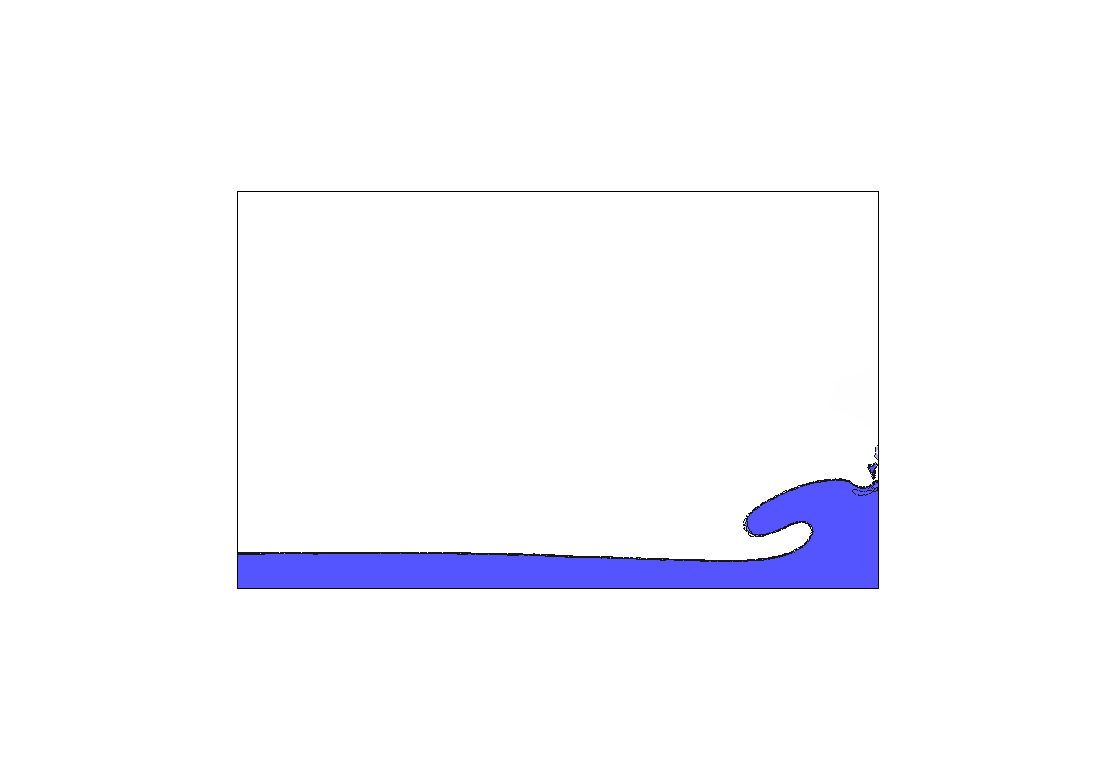
\includegraphics[width=0.275\textwidth, trim=7.5cm 6.5cm 7.5cm 6.5cm, clip=true]{./water_collapse/water_collapse_300.png}}
\subfigure[$t=1.75$]{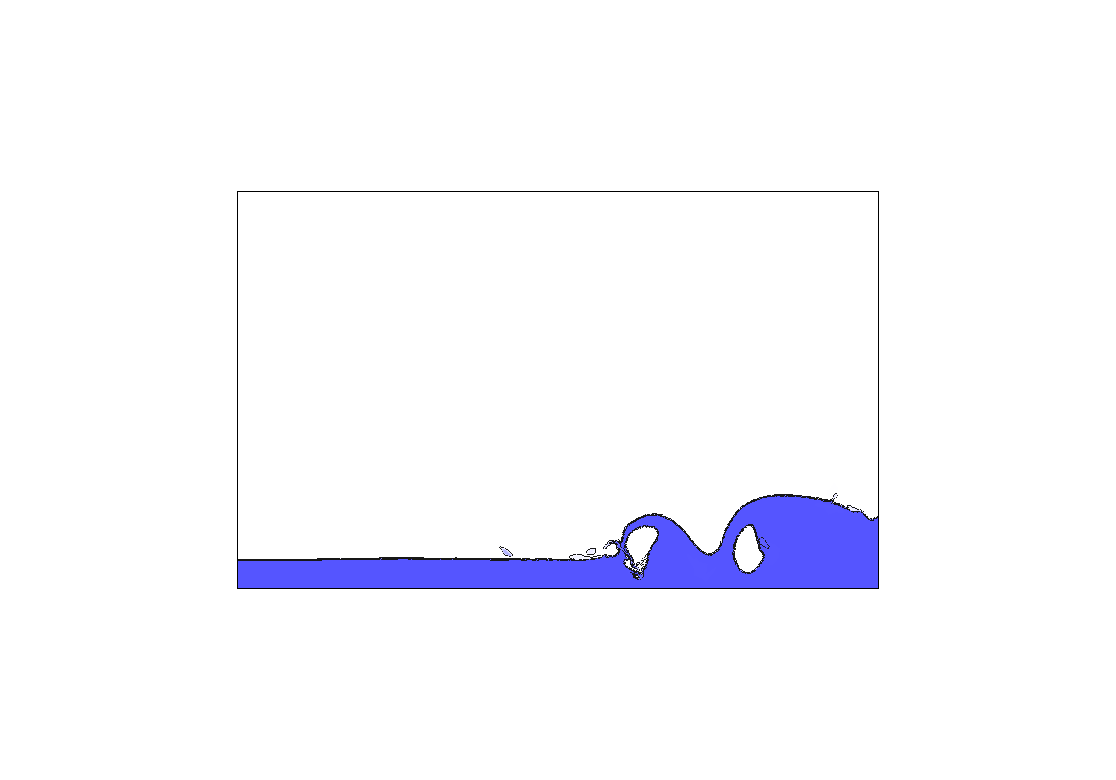
\includegraphics[width=0.275\textwidth, trim=7.5cm 6.5cm 7.5cm 6.5cm, clip=true]{./water_collapse/water_collapse_350.png}}
\subfigure[$t=2.25$]{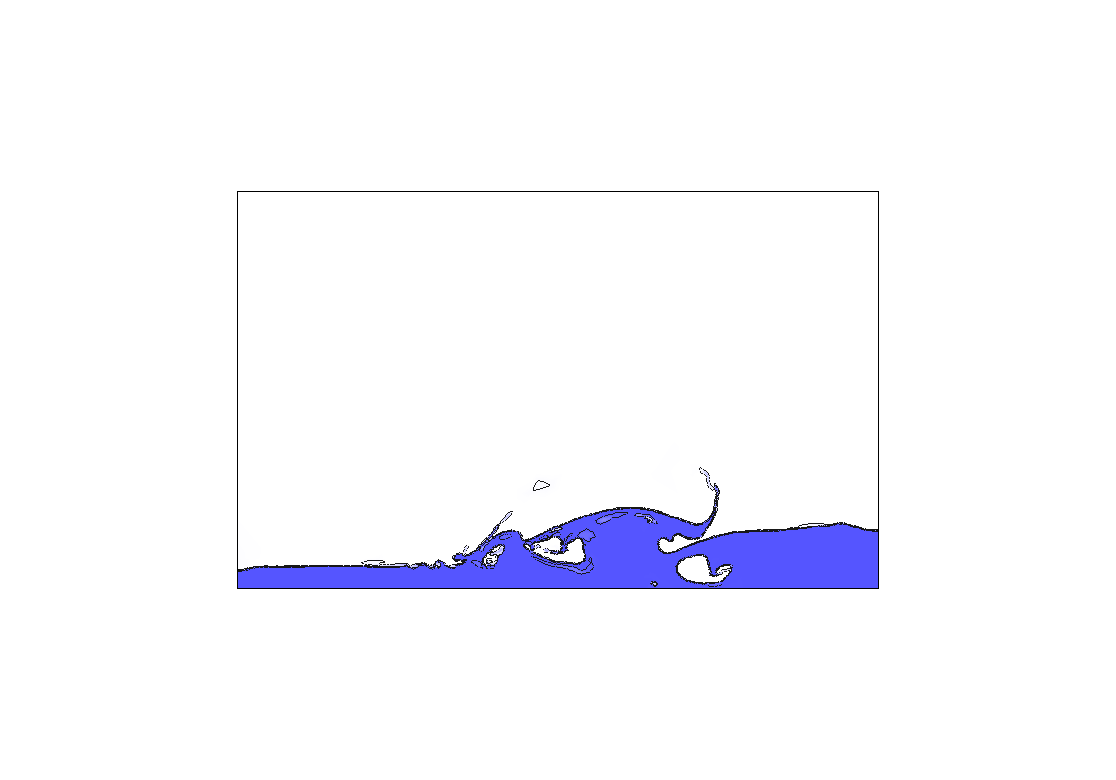
\includegraphics[width=0.275\textwidth, trim=7.5cm 6.5cm 7.5cm 6.5cm, clip=true]{./water_collapse/water_collapse_450.png}}
\subfigure[$t=2.5$]{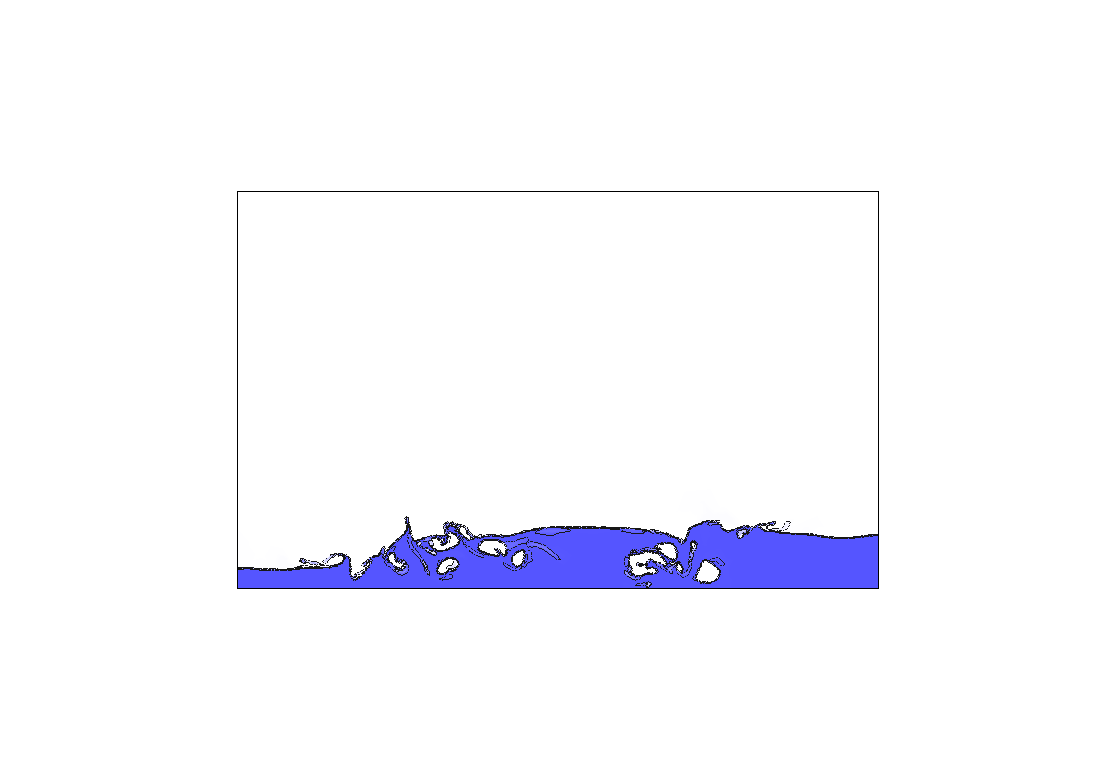
\includegraphics[width=0.275\textwidth, trim=7.5cm 6.5cm 7.5cm 6.5cm, clip=true]{./water_collapse/water_collapse_500.png}}
\caption{The evolution of the water volume fraction over several timesteps.  The presence of water is indicated as a blue region and the interface to the air is delineated by the contours (in black).}
\end{figure}

\end{frame}
%
\begin{frame}
    \frametitle{Water collapse}
\begin{itemize}
\item Post--processing scripts output several plots, e.g. comparison of water depth to experimental data
\end{itemize}
\begin{figure}
\centering
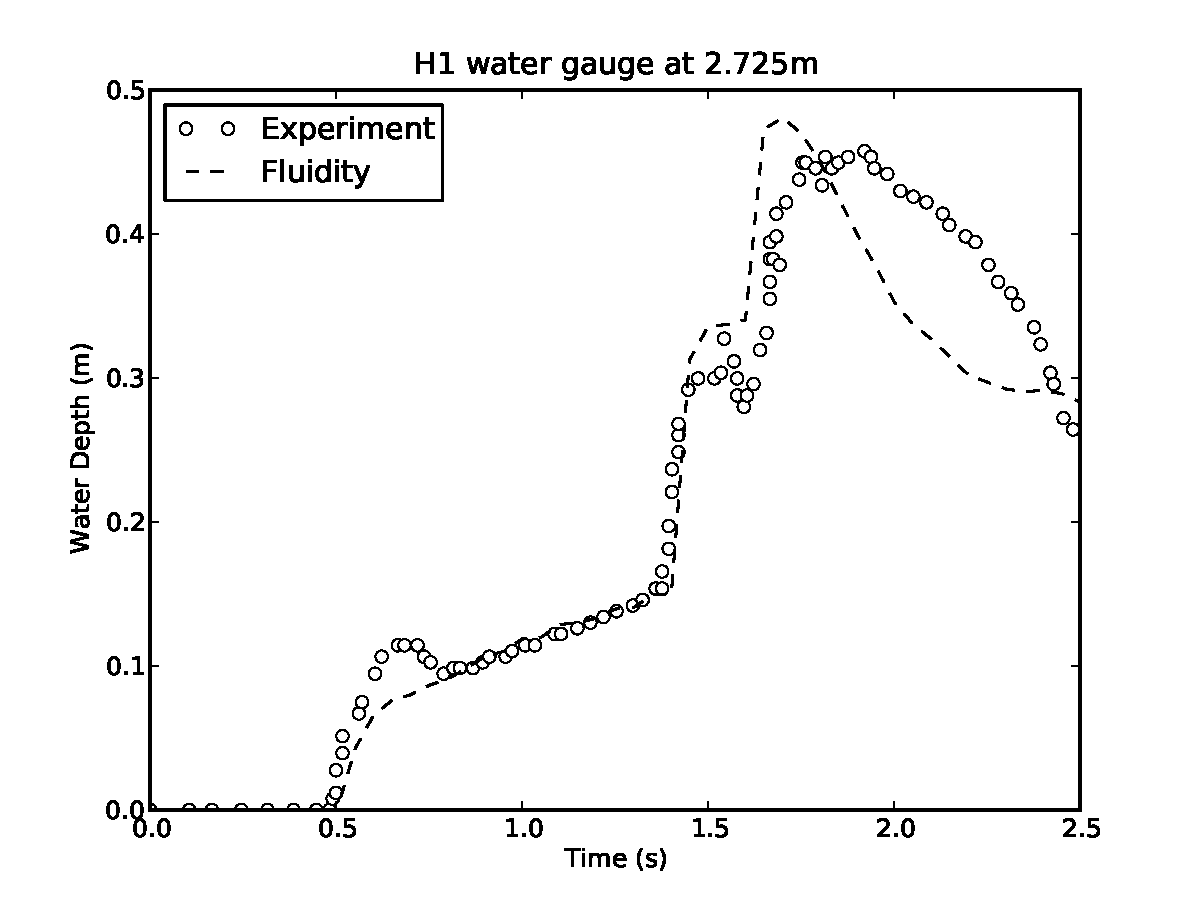
\includegraphics[width=0.5\textwidth]{./water_collapse/water_gauge_H1.pdf}
\caption{Comparison with experimental depth gauge data at $x = 2.725 \, $m.}
\end{figure}

\end{frame}
%
\begin{frame}
    \frametitle{Water collapse, exercises}
\begin{itemize}
\item Disable the adaptivity option to run on a fixed mesh.
\item Alter the water/air viscosity/density.
\item Modify the tank geometry.
\end{itemize}

\end{frame}

%-- Add sections and your outline will be created automatically --%
\subsection{Tephra settling}

% Frame starts a new slide
\begin{frame}
  \frametitle{Tephra settling}
  \begin{itemize}
  \item Replicates a laboratory experiment of tephra (fine volcanic ash particles) settling through a tank of water
    (Carey, 1997)
  \item Small tephra particles can settle either individually according to Stokes' law, or collectively as a cloud of particles (a plume)
  \item Dispersed multiphase approach, adaptive timestepping
  \item Run time: 1 hr.
    % \item Plumes are generated when the bulk density of the tephra-water mixture becomes large enough, yielding settling velocities much greater than those expected of single particles (which settle at a velocity given by Stokes law).
  \end{itemize}
\end{frame}

% \begin{frame}
%   \frametitle{Tephra settling - Simulation setup}
%   \begin{itemize}
%     \item The simulation uses a 0.3 x 0.7 metre domain, replicating the cross-section of the water tank used in the experiments.
%     \item No normal flow boundary conditions are weakly imposed along with a zero velocity initial condition, and the initial volume fraction of the particle phase is set to $1.0 \times 10^{-7}$.
%     \item The influx of particles from the air above is simulated using a \texttt{flux} boundary condition at the top of the domain. This allows tephra to flux in at a rate of $0.472\ \mathrm{gm^{-2}s^{-1}}$.
%   \end{itemize}
% \end{frame}

\begin{frame}
  \frametitle{Tephra settling - Numerical results (1)}
\begin{figure}[H]
        \centering
                
\includegraphics[scale=0.2]{tephra_settling/tephra_fine_1.png}\hspace{0.1cm}
                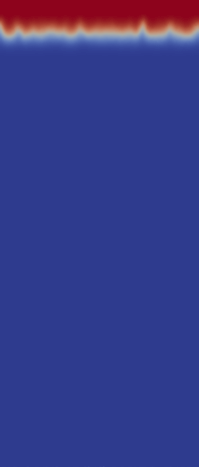
\includegraphics[scale=0.2]{tephra_settling/tephra_fine_2.png}\hspace{0.1cm}
                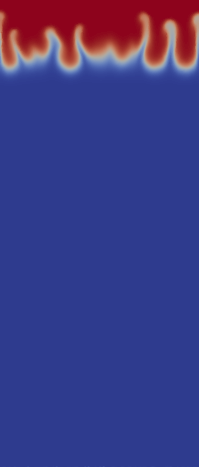
\includegraphics[scale=0.2]{tephra_settling/tephra_fine_3.png}\hspace{0.1cm}
                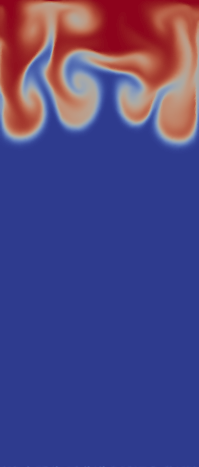
\includegraphics[scale=0.2]{tephra_settling/tephra_fine_4.png}\hspace{0.1cm}
                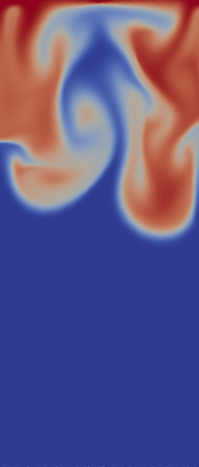
\includegraphics[scale=0.2]{tephra_settling/tephra_fine_5.png}
   \label{fig:tephra_adaptive}
   \caption{Simulation visualisations at $t = 10, 30, 50, 80$ and $110$ seconds. Tephra particles initially settle individually, but as more tephra fluxes in, the layer eventually becomes unstable and plumes begin to form.}
\end{figure}
\end{frame}

\begin{frame}
  \frametitle{Tephra settling - Numerical results (2)}
\begin{figure}[H]
        \centering
                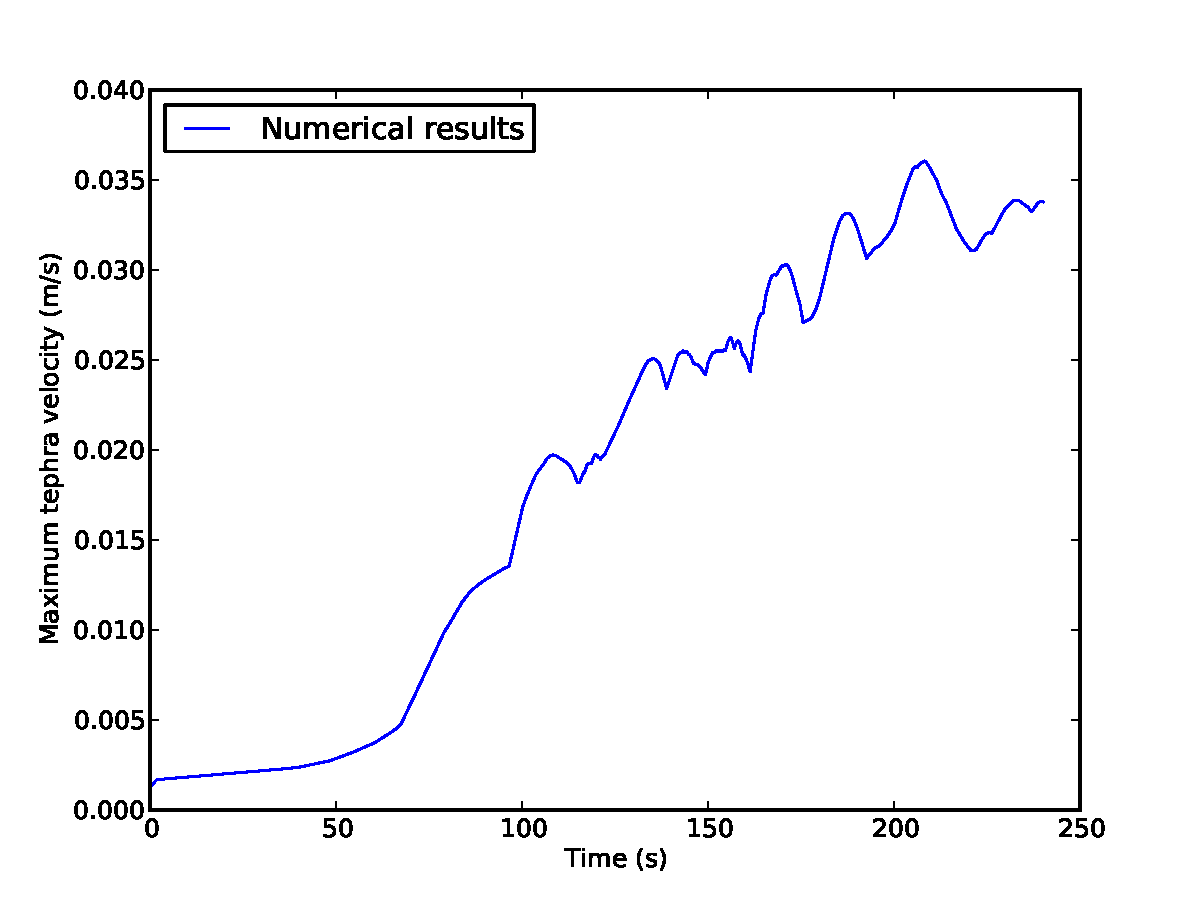
\includegraphics[scale=0.27]{tephra_settling/tephra_velocity.pdf}
   \label{fig:tephra_velocity}
   \caption{Plot of the maximum tephra phase velocity against time. Tephra particles initially settle at approximately $0.0017\ \mathrm{ms^{-1}}$, as predicted by Stokes' law. Plumes begin to form after approximately 30 seconds, resulting in settling velocities over 10 times greater than that of an individual particle.}
\end{figure}
\end{frame}

\begin{frame}
  \frametitle{Tephra settling - Exercises}
 \begin{itemize}
    \item Decrease the characteristic element size to better resolve the plume behaviour.\newline
    \item Alter the particle size to observe its effect on plume formation.\newline
    \item Add a second particle phase (with a different particle size).
 \end{itemize}
\end{frame}




%-- Data directory slide --- %
\section*{Data}
\begin{frame}
  \frametitle{Data}
  \begin{center}
  The examples have been run in advance \\ and the output can be found in \\ /scratch/release-examples
  \end{center}
\end{frame}
\end{document}




